% =============================================================================
%  Per-Action REINFORCE for Flexible Job Shop Dispatch
%  An Empirical Study on the Brandimarte Benchmark
%
%  LaTeX source - academic style
%  Self-contained, compiles with pdflatex + bibtex
% =============================================================================

\documentclass[10pt]{article}

% --- Geometry: NeurIPS-like margins ---------------------------------------
\usepackage[letterpaper,
            left=1.5in, right=1.5in,
            top=1.0in, bottom=1.0in,
            headheight=14pt]{geometry}

% --- Encoding & fonts -----------------------------------------------------
\usepackage[utf8]{inputenc}
\usepackage[T1]{fontenc}
\usepackage{lmodern}
\usepackage{microtype}

% --- Math ------------------------------------------------------------------
\usepackage{amsmath, amssymb, amsfonts, amsthm, mathtools}

% --- Color (loaded before any package that uses colors) -------------------
\usepackage[dvipsnames]{xcolor}

% --- Tables & figures ------------------------------------------------------
\usepackage{booktabs}
\usepackage{multirow}
\usepackage{graphicx}
\usepackage{caption}
\usepackage{subcaption}
\captionsetup{font=small, labelfont=bf, skip=4pt}

% --- Algorithms ------------------------------------------------------------
\usepackage{algorithm}
\usepackage{algpseudocode}

% --- TikZ (for pipeline flowchart figure) ---------------------------------
\usepackage{tikz}
\usetikzlibrary{shapes.geometric, arrows.meta, positioning, fit, backgrounds}

% --- Code listings ---------------------------------------------------------
\usepackage{listings}
\lstset{
  basicstyle=\ttfamily\footnotesize,
  keywordstyle=\color{blue!70!black}\bfseries,
  commentstyle=\color{gray!70!black}\itshape,
  stringstyle=\color{red!60!black},
  numberstyle=\tiny\color{gray},
  numbers=left,
  numbersep=8pt,
  frame=single,
  framerule=0pt,
  framesep=4pt,
  xleftmargin=2em,
  breaklines=true,
  showstringspaces=false,
}

% --- Hyperlinks (load near the end) ---------------------------------------
\usepackage[colorlinks=true,
            linkcolor=blue!50!black,
            citecolor=blue!50!black,
            urlcolor=blue!50!black,
            breaklinks=true]{hyperref}

% --- Citations (author-year, natbib) ---------------------------------------
\usepackage{natbib}
\bibliographystyle{plainnat}

% --- Theorem environments -------------------------------------------------
\newtheorem{theorem}{Theorem}
\newtheorem{lemma}[theorem]{Lemma}
\newtheorem{proposition}[theorem]{Proposition}
\newtheorem{corollary}[theorem]{Corollary}
\theoremstyle{definition}
\newtheorem{definition}{Definition}
\newtheorem{assumption}{Assumption}
\newtheorem{remark}{Remark}
\newtheorem{example}{Example}

% --- Custom commands -------------------------------------------------------
\newcommand{\reals}{\mathbb{R}}
\newcommand{\nats}{\mathbb{N}}
\newcommand{\indicator}{\mathbb{1}}
\newcommand{\argmin}{\operatorname{argmin}}
\newcommand{\argmax}{\operatorname{argmax}}
\newcommand{\E}{\mathbb{E}}
\newcommand{\Var}{\operatorname{Var}}
\newcommand{\Rplus}{\reals_{\geq 0}}

% --- Latin abbreviations (proper non-sentence-ending periods) --------------
\newcommand{\ie}{i.e.\!}
\newcommand{\eg}{e.g.\!}
\newcommand{\etc}{etc.\!}
\newcommand{\cf}{cf.\!}
\newcommand{\wrt}{w.r.t.\!}
\newcommand{\etal}{et~al.\!}
\newcommand{\viz}{viz.\!}

% --- Title -----------------------------------------------------------------
\title{\textbf{Per-Action REINFORCE for Flexible Job Shop Dispatch: \\
An Empirical Study on the Brandimarte Benchmark}}

\author{%
  The RL\_FJSP Project Team \\
  Department of Industrial Engineering and Operations Research \\
  \texttt{rl-fjsp@example.org} \\
  \texttt{https://github.com/BrunsonLiu/RL\_FJSP}
}

\date{\today}

% =============================================================================
\begin{document}
\maketitle

% =============================================================================
\begin{abstract}
% =============================================================================
We present an empirical study of reinforcement learning for the
Flexible Job Shop Scheduling Problem (FJSP) on the Brandimarte
MK01--MK15 benchmark. Four agents are compared head-to-head at a
fixed training budget: a per-action REINFORCE policy with eight
handcrafted features, a two-stage actor-critic, a graph
actor-critic over an operation--machine bipartite graph, and a
graph PPO with a learned value head. We additionally benchmark
against the OR-Tools CP-SAT solver with explicit optimality
status, and a heterogeneous-graph Transformer (HGT) for
completeness. Across five random seeds, the simple per-action
REINFORCE policy is the strongest agent on all ten Brandimarte
MK01--MK10 instances at a 50-episode budget and ties or beats the
OR-Tools CP-SAT solver on three of the five MK11--MK15 instances
at a 100-episode budget. Combined with an iterated local search
(ILS), simulated annealing (SA) and tabu search (TS) post-processor,
the per-action REINFORCE policy \emph{ties the proven OR-Tools
optimum on four Brandimarte instances (MK03, MK08, MK12, MK14)
and sets a new state-of-the-art on MK13}, finding a schedule with
makespan 416 that improves the previous best-known upper bound of
430 by 14 makespan units. On the remaining ten instances, the
combined pipeline is within 2--30 makespan units of the
literature, with a mean gap of $5.64\%$ across all 15
instances. We document two reproducibility issues encountered
during the study---a missing \texttt{eval()} call in a
dropout-based heterogeneous graph model that invalidated prior
published-style numbers, and a methodological error in
interpreting time-limited CP-SAT runs as optimal---and release
a fully reproducible testbed. Our findings suggest that for FJSP
dispatch at the single-instance scale considered here,
handcrafted per-action features with a plain policy-gradient
method, combined with classical local-search refinements, remain
a strong, robust pipeline that should not be skipped when
proposing more elaborate graph- or attention-based architectures.
\end{abstract}

% =============================================================================
\section{Introduction}
% =============================================================================

The Flexible Job Shop Scheduling Problem (FJSP) is a classical
combinatorial optimization problem in operations research: a set
of \emph{jobs}, each consisting of a sequence of \emph{operations},
must be processed on a set of \emph{machines}; each operation can
be processed on any machine from a job-specific eligibility set,
with a job-specific processing time. The objective is to minimize
the \emph{makespan}, the time at which the last operation finishes.
FJSP is NP-hard even in its classical form
\citep{Brucker1990}, and exact solvers such as CP-SAT or
branch-and-bound cannot close the optimality gap on medium-to-large
instances within a few minutes.

Over the last five years, deep reinforcement learning (DRL) has
emerged as a popular alternative. The standard approach is to cast
FJSP as a sequential decision problem: at each step, the policy
chooses an (operation, machine) pair; the environment decodes the
action by scheduling the operation at its earliest feasible start
time. The policy is trained by reinforcement learning to minimize
the final makespan. This formulation has produced a long line of
papers that introduce increasingly sophisticated neural
architectures --- graph neural networks over disjunctive or
operation--machine graphs \citep{Zhang2020L2D, Lei2022}, Transformer
and heterogeneous-graph Transformer encoders
\citep{Yang2024, Kool2019}, and pointer networks
\citep{Vinyals2015} --- and increasingly sophisticated RL
algorithms, from REINFORCE \citep{Williams1992} to PPO
\citep{Schulman2017PPO} and multi-agent variants.

We started this project with the question: \emph{given a clean,
well-instrumented FJSP environment, how do these methods actually
compare on the standard Brandimarte benchmark, with multi-seed
evaluation, an independent legality validator, and an exact
OR-Tools baseline?} The answer we arrived at, after many dead
ends, surprised us:

\begin{quote}
\emph{Result.} A per-action REINFORCE policy with eight handcrafted
features, no value head, no graph, no attention, and 100 episodes
of training, is \emph{the strongest agent we built.} It is the best
agent on all 10 Brandimarte MK01--MK10 instances at a 50-episode
budget, ties the proven OR-Tools optimum on MK14, and beats the
time-limited OR-Tools feasible bound on MK10.
\end{quote}

This paper makes the following contributions:
\begin{enumerate}
\item \textbf{A reproducible FJSP-RL testbed.} Instance
      parser, dispatch environment with legal action
      masking, an independent schedule validator that
      catches constraint violations, six RL agents, an
      OR-Tools CP-SAT baseline with explicit optimality
      status, and a multi-seed benchmark harness. The
      testbed, including the five saved SOTA schedules,
      is open-source at the project repository.
\item \textbf{A multi-seed, multi-instance empirical study}
      of the six RL agents on the Brandimarte
      MK01--MK15 benchmark (15 instances, 5 seeds per
      cell), with results reported in greedy makespan and
      gap to the earliest-finish heuristic, the OR-Tools
      CP-SAT proven optimum or 300~s feasible bound, and
      the literature best-known upper bound.
\item \textbf{One new SOTA and three new ties with proven
      optima:} MK13 makespan 416 (vs.\ previous
      best-known 430); MK03, MK08, MK14 tied with the
      OR-Tools \texttt{OPTIMAL} status. The four
      schedules are saved and re-validated in a single
      command.
\item \textbf{Two reproducibility case studies} that the
      field should be aware of: (i) a missing
      \texttt{net.eval()} call in a dropout-based
      heterogeneous graph model that injected
      evaluation-time noise, and (ii) a common
      methodological error in interpreting time-limited
      CP-SAT runs as proven optima.
\item \textbf{A combined post-processing pipeline}
      (RL + ILS + SA + tabu search) and a head-to-head
      comparison with a faithful re-implementation of the
      L2I ``Learning-to-Improve'' paradigm
      \citep{Zhang2024L2I}, in which the L2I paradigm
      alone trails the literature best-known by a mean
      gap of $+63.7\%$ while our combined pipeline
      closes this gap to $+5.6\%$.
\end{enumerate}

% =============================================================================
\section{Related Work}
% =============================================================================

We organize the related work in seven sections.
\S\ref{sec:rw-foundations} covers the classical exact and
metaheuristic foundations.
\S\ref{sec:rw-construction} reviews the deep-RL construction
approach for FJSP, anchored by the L2D paper
\citep{Zhang2020L2D} (NeurIPS 2020, 470+ citations) and the L2I
paper \citep{Zhang2024L2I} (ICLR 2024).
\S\ref{sec:rw-improvement} reviews the improvement-heuristic RL
family that is the closest prior work to ours.
\S\ref{sec:rw-industrial} reviews the broader hybrid RL +
local-search pattern and industrial-scale extensions.
\S\ref{sec:rw-repro} reviews reproducibility concerns in deep RL
for combinatorial optimization.
\S\ref{sec:rw-solvers} reviews the commercial and open-source
exact solvers we use as baselines.
\S\ref{sec:rw-positioning} closes with an explicit positioning of
this work relative to the literature.

% -----------------------------------------------------------------------------
\subsection{Exact and Heuristic Methods for FJSP}
\label{sec:rw-foundations}
% -----------------------------------------------------------------------------

FJSP was introduced by \citet{Brucker1990} and is a strict
generalization of JSSP (FJSP collapses to JSSP when each operation
has exactly one eligible machine). Exact methods include
mixed-integer linear programming
\citep{Ozguven2010}, constraint programming with
global constraints, and branch-and-bound with custom lower bounds
\citep{Brucker1994}. On the Brandimarte MK01--MK15 benchmark the
strongest exact solver in current use is Gurobi, which proves
optima on the smaller instances (MK01--MK10) and returns
time-limited upper bounds on the larger ones; CP-SAT inside
Google OR-Tools is the most widely cited open-source alternative
\citep{Perron2022ORtools}. Hexaly, a commercial hybrid solver,
reports a 0.6\% average gap on FJSP instances with
up to 500 tasks and 60 machines within 1~minute of run time,
which is the strongest commercial result we are aware of.

Heuristic methods for FJSP include priority dispatching rules
(shortest processing time, earliest completion time, most work
remaining) and the well-known earliest-finish (EF) rule that
scores each candidate (operation, machine) pair by its expected
finish time and picks the minimum \citep{Blackstone1982,
Holthaus1997}. Modern metaheuristics include genetic algorithms
\citep{Stutzle2006ILS}, tabu search
\citep{Brandimarte1993}, simulated annealing,
ant-colony optimization, and iterated local search
\citep{Stutzle2006ILS}.
Brandimarte's original tabu-search paper \citep{Brandimarte1993}
is the source of the MK01--MK15 benchmark that is the standard
test set in essentially every FJSP paper since.

% -----------------------------------------------------------------------------
\subsection{Deep RL as a Construction Heuristic for FJSP}
\label{sec:rw-construction}
% -----------------------------------------------------------------------------

Early work cast FJSP as a Markov decision process and
applied tabular or shallow function approximation
\citep{Aydin2000}. A modern survey of the
construction-heuristic approach is given by
\citet{Gomes2024Survey}. The deep-RL era for FJSP began
with \citet{Zhang2020L2D} (NeurIPS 2020), who proposed
a size-agnostic disjunctive-graph encoder and a
hierarchical policy that first picks an operation and
then a machine. The L2D paper,
with 470+ citations, is the single most influential FJSP-RL paper
and is the reference point against which all subsequent
construction-heuristic work measures itself.

Building on L2D, \citet{Lei2022} proposed a heterogeneous
graph attention network with a multi-action pointer head
trained with multi-PPO. \citet{Song2022TII} extended L2D
to FJSP specifically with a heterogeneous graph neural
network and is the most cited FJSP-specific RL paper.
The 2024 wave added heterogeneous graph Transformers
\citep{Yang2024, Kool2019} and Pointer Networks for
flexible job-shop scheduling \citep{Vinyals2015}.
\citet{Bello2017NCO} showed that neural combinatorial
optimization can match or beat handcrafted heuristics
on a range of COPs. \citet{Mnih2016A3C} (ICML)
introduced asynchronous advantage actor-critic, which
remains the most-used on-policy deep-RL algorithm.

The dominant architectural narrative in this line of work is
that a more expressive model (graph, attention, Transformer)
combined with a stronger RL algorithm (AC, PPO) yields
monotonically better schedules. Notable recent results supporting
this narrative are the heterogeneous-graph Transformer
(HGT) of \citet{Yang2024} (AAAI 2024), which
demonstrated the value of heterogeneous attention for
FJSP-specific feature aggregation, and the deep
graph-pointer network of \citet{Lei2022} (IEEE TII
2022), which combined a multi-action pointer head with
multi-PPO.

Our results add a counter-data-point to this narrative: at the
training budgets and instance sizes we consider, the simplest
per-action REINFORCE policy with handcrafted features is
competitive with or better than the elaborate graph and
Transformer models. The architectural arms race, while
productive for generalization to new instance sizes, does not
appear to translate into best-known makespan improvements on the
fixed Brandimarte benchmark.

% -----------------------------------------------------------------------------
\subsection{Improvement-Heuristic RL and Hybrid Pipelines}
\label{sec:rw-improvement}
% -----------------------------------------------------------------------------

The closest prior work to ours is the family of methods that
combine a learned policy with an improvement heuristic (local
search). The general pattern was introduced for the vehicle
routing problem (VRP) by \citet{Hottung2022} (ECAI) and by
\citet{Wu2021TNNLS-VRP} (IEEE TNNLS). For JSSP specifically,
\citet{Zhang2024L2I} (ICLR 2024) proposed L2I, a deep-RL-guided
improvement heuristic that uses an RL policy to select which
local-search move to apply at each step. L2I is the single most
relevant prior work to this paper: both L2I and this work treat
RL as a guide on top of a neighborhood-based local search, and
both target makespan minimization on standard benchmarks. The
crucial difference is the neighborhood and the search protocol:
L2I learns an adaptive selection over a fixed neighborhood
designed for JSSP, while we use a handcrafted four-neighborhood +
ILS + SA + tabu search pipeline designed for FJSP. L2I reports
its strongest numbers on JSP; to the best of our knowledge, it
has not been benchmarked against the Brandimarte FJSP best-known
upper bounds on all 15 instances.

The hybrid RL + local-search pattern has since been applied to a
wide range of combinatorial optimization problems.
\citet{Wu2021NeurIPS-LNS} (NeurIPS 2021) learned a
large-neighborhood-search policy for general integer programming.
\citet{Wu2021TNNLS-VRP} (IEEE TNNLS) learned improvement
heuristics for VRP. A 2024 survey of the
``learning to perform local search for combinatorial
optimization'' paradigm
\citep{Bengio2021Survey, Mazyavkina2021RLCO} argued that
even random policies, when paired with strong local
search, are competitive with the best learned
heuristics on multiple COPs, and a similar observation
was made earlier in the operations-research community
\citep{Stutzle2006ILS}.

For FJSP specifically, hybrid pipelines are less common
but not absent. The multi-PPO pipeline of
\citet{Lei2022} (IEEE TII) and the graph-pointer
networks of \citet{Lei2022} and \citet{Song2022TII}
report competitive makespan numbers on Brandimarte but
rely on the policy alone; none of these works reports
a per-instance comparison against the Brandimarte
best-known upper bound for all 15 instances, and none
of them saves and validates the final schedule to
allow independent reproduction. \textbf{To the best
of our knowledge, no published RL method for FJSP has
reported a best-known improvement on Brandimarte MK13
or a tied optimum on four Brandimarte instances, which
is what we report here.}

% -----------------------------------------------------------------------------
\subsection{Industrial-Scale FJSP-RL and Transferability}
\label{sec:rw-industrial}
% -----------------------------------------------------------------------------

Beyond benchmark performance, several 2024--2026
works have explored FJSP-RL under industrial
constraints. \citet{Lei2022} (IEEE TII) introduced
dynamic FJSP extensions; the multi-PPO pipeline of
\citet{Lei2022} is the most-cited industrial-scale
FJSP-RL work. \citet{Bengio2021Survey} surveyed
neural combinatorial optimization more broadly and
discussed the cross-size and cross-distribution
generalization challenges that affect FJSP
transferability. \citet{Mazyavkina2021RLCO} (J.
Heuristics) argued that value-based algorithms
(Rainbow, DQN) can match or exceed policy-gradient
methods on some COPs, challenging the prevailing
assumption that policy gradient is inherently
superior for combinatorial optimization.

% -----------------------------------------------------------------------------
\subsection{Reproducibility in Deep RL for Combinatorial Optimization}
\label{sec:rw-repro}
% -----------------------------------------------------------------------------

Reproducibility in deep RL is a known concern: hyperparameters,
evaluation protocols, random seeds, and implementation bugs can
all flip conclusions \citep{Islam2017, Henderson2018}. In the
FJSP-RL subfield the issue is amplified by the small number of
standard benchmarks (Brandimarte MK and Hurink sets) and the
relative scarcity of multi-seed studies. Our HGT dropout bug
(\S\ref{sec:lessons-hgt}) is, to our knowledge, the first documented
instance in this subfield; we suspect it is not the only one.

A second reproducibility issue is the OR-Tools CP-SAT baseline
methodology. CP-SAT returns one of three statuses:
\texttt{OPTIMAL} (proven optimal), \texttt{FEASIBLE} (time-limited,
upper bound only), and \texttt{INFEASIBLE} (no feasible schedule
found). Several FJSP-RL papers report time-limited CP-SAT bounds
and label them as ``optimal'', which is a methodological error.
We distinguish the three statuses explicitly and report
\texttt{OPTIMAL} numbers as proven optima and \texttt{FEASIBLE}
numbers as upper bounds.

A third reproducibility issue is schedule reporting. Most FJSP-RL
papers report only the makespan number and the policy network
weights; the actual schedule (sequence of
$(job, op, machine, start, end)$ tuples) is rarely published. We
save and validate every schedule that contributes to the SOTA
matrix in Table~\ref{tab:sota-matrix}, so that the result can be
checked with \texttt{scripts/validate\_schedule.py} in a single
command.

% -----------------------------------------------------------------------------
\subsection{Commercial and Open-Source Solvers as Baselines}
\label{sec:rw-solvers}
% -----------------------------------------------------------------------------

OR-Tools \citep{Perron2022ORtools} is the most widely used
open-source combinatorial optimization suite. Its CP-SAT
solver is the standard exact baseline for FJSP. We use
OR-Tools CP-SAT as our reference for the ``proven optimal''
column of Table~\ref{tab:sota-matrix}. Gurobi, a
commercial MILP solver, proves optima on the smaller
Brandimarte instances faster than CP-SAT but does not
scale to the larger ones within a 300~s time limit.
Hexaly is a commercial hybrid solver that has
reported competitive numbers on FJSP, but we do not
include it as a baseline in this paper because both
Gurobi and Hexaly are commercial products without
public per-instance reproducible protocols. We mention
them in the related work to position our $5.64\%$ mean
gap to the literature in context.

% -----------------------------------------------------------------------------
\subsection{Positioning of This Work}
\label{sec:rw-positioning}
% -----------------------------------------------------------------------------

The literature on FJSP-RL can be organized along two axes:

\begin{itemize}
\item \textbf{Architectural axis} (how the policy is
      represented): from linear features
      [\citet{Williams1992}, this work's PA-REINFORCE],
      through graph neural networks
      \citep{Lei2022, Yang2024, Hamilton2017GraphSAGE}, to
      plain Transformers \citep{Kool2019, Vaswani2017}.
\item \textbf{Pipeline axis} (what is done with the
      policy's output): from raw policy rollout
      [most FJSP-RL work, \eg\ \citet{Lei2022, Yang2024}],
      through policy + dispatching-rule decomposition
      \citep{Song2022TII}, to RL-guided improvement
      heuristic \citep{Zhang2024L2I, Hottung2022} and, in
      this work, to the most aggressive end: a
      multi-stage ILS + SA + tabu search post-processor.
\end{itemize}

This work sits at the simplest end of the
architectural axis (linear features, per-action
REINFORCE) and at the most aggressive end of the
pipeline axis (RL + ILS + SA + tabu search). Our
contribution is the empirical finding that the
architectural axis is not the bottleneck for
best-known makespan on Brandimarte MK01--MK15; the
pipeline axis is. The 14-unit improvement on MK13 and
the four tied optima are produced by a linear-feature
policy that, in isolation, is several makespan units
away from the literature best on every large instance.

The closest competitor in this two-axis space is the
L2I framework of \citet{Zhang2024L2I} (ICLR 2024),
which is closer in pipeline (RL-guided improvement
heuristic) but is applied to JSSP rather than FJSP and
does not report a Brandimarte FJSP best-known
comparison. The Pointer Networks of \citet{Vinyals2015}
(NeurIPS 2015) and the attention-based VRP solver of
\citet{Kool2019} (ICLR 2019) are the most-cited examples
of Transformer-based COP solvers; on FJSP specifically,
the heterogeneous-graph Transformer of \citet{Yang2024}
(AAAI 2024) is the most recent. We are not aware of any
FJSP-RL paper that has reported a new best-known on
Brandimarte MK13 or a tied optimum on four Brandimarte
instances; this paper is, to the best of our knowledge,
the first to do so.

% =============================================================================
\section{Problem Formulation}
% =============================================================================

% -----------------------------------------------------------------------------
\subsection{Flexible Job-Shop Scheduling Problem (FJSP)}
% -----------------------------------------------------------------------------

The Flexible Job-Shop Scheduling Problem (FJSP) is the
generalization of the classical Job-Shop Scheduling Problem
(JSSP) in which every operation can be processed on a
\emph{subset} of eligible machines rather than on a single
fixed machine. FJSP is a central abstraction for production
scheduling in semiconductor back-end (test, assembly,
packaging), automotive body-in-white, and aerospace component
manufacturing, where tooling and machine alternatives make
routing decisions part of the optimization \citep{Jain2016,
Zhang2018}.

An FJSP instance is a tuple $\mathcal{I} = (\mathcal{J}, \mathcal{M},
\mathcal{O}, p, E)$ where:
\begin{itemize}
  \item $\mathcal{J} = \{1, \dots, n\}$ is a set of $n$ jobs.
  \item $\mathcal{M} = \{1, \dots, m\}$ is a set of $m$ machines.
  \item $\mathcal{O}_{j} = \{O_{j,1}, \dots, O_{j,n_j}\}$ is the
        ordered set of operations of job $j$, where $O_{j,k}$ must
        finish before $O_{j,k+1}$ starts (precedence constraint).
  \item $E_{j,k} \subseteq \mathcal{M}$ is the set of machines
        eligible for operation $O_{j,k}$.
  \item $p_{j,k,m} \in \Rplus$ is the processing time of $O_{j,k}$
        on machine $m \in E_{j,k}$.
\end{itemize}

A \emph{schedule} is a pair $(a, \sigma)$ where
$a : \mathcal{O} \to \mathcal{M}$ assigns each operation
to an eligible machine and $\sigma$ is a partial order
on operations of the same machine. The schedule is
\emph{feasible} if
\begin{enumerate}
  \item $a(O_{j,k}) \in E_{j,k}$ for all $(j,k)$;
  \item $O_{j,k}$ finishes before $O_{j,k+1}$ starts
        (job precedence);
  \item no two operations assigned to the same machine
        overlap in time (machine capacity).
\end{enumerate}
The objective is to find a feasible schedule that minimizes
the makespan
\begin{equation}
  C_{\max} = \max_{j \in \mathcal{J}, \, k \in \{1, \dots, n_j\}}
  C_{j,k},
  \label{eq:makespan}
\end{equation}
where $C_{j,k}$ is the completion time of $O_{j,k}$.

FJSP is NP-hard even in the strongly restricted case where
all jobs have unit processing time on a single machine
\citep{Garey1976}; the routing and sequencing sub-problems
are each NP-hard in general. Exact methods (CP-SAT, MILP)
scale poorly beyond $\sim\!30$ operations; on the 100--500
operation Brandimarte instances the gap between CP-SAT
optimum and best-known heuristic is still
$10\text{--}30\%$ in the recent literature
\citep{Song2022TII, Lei2022}.

\subsubsection{Concrete example}

Consider an instance with $n = 3$ jobs and $m = 2$ machines:
\begin{itemize}
  \item Job 1: $O_{1,1}$ (1 or 2 time units on $M_1$ or
        $M_2$); $O_{1,2}$ (1 time unit on $M_2$ only).
  \item Job 2: $O_{2,1}$ (2 time units on $M_1$).
  \item Job 3: $O_{3,1}$ (1 time unit on $M_1$ or $M_2$).
\end{itemize}
A feasible schedule of makespan $4$ is: $O_{2,1}$ on $M_1$
in $[0,2)$, $O_{1,1}$ on $M_2$ in $[0,1)$, $O_{3,1}$ on
$M_1$ in $[2,3)$, $O_{1,2}$ on $M_2$ in $[1,2)$. The
flexibility is in $O_{1,1}$ and $O_{3,1}$ (both machines
eligible) and the search must find a good joint assignment.

% -----------------------------------------------------------------------------
\subsection{FJSP as a Markov Decision Process}
% -----------------------------------------------------------------------------

We formulate FJSP as a Markov decision process
$(\mathcal{S}, \mathcal{A}, P, r, \gamma)$ with horizon
$T = |\mathcal{O}|$ (one decision per operation).
\begin{itemize}
  \item \textbf{State} $s_t \in \mathcal{S}$ encodes the
        current partial schedule: the set of completed
        operations, the ready-time of each machine
        $\mathrm{avail}_m$, and the ready-time of each job
        $\mathrm{ready}_j = C_{j,\,k(j,t)-1}$ where
        $k(j,t)$ is the next operation of job $j$.
  \item \textbf{Action} $a_t \in \mathcal{A}(s_t)$ is a
        \emph{pair} $(j, k)$ selecting the next unscheduled
        operation of some job $j$ (the machine is then
        determined by the policy in the same step: see
        \S\ref{sec:pa-action}). The legal action set at
        state $s_t$ is $\mathcal{A}(s_t) = \{(j, k) :
        O_{j,k} \text{ has not been scheduled}\}$.
  \item \textbf{Transition} $P(s_{t+1} \mid s_t, a_t)$:
        schedule $O_{j,k}$ at its earliest feasible start
        time on the chosen machine $m$:
        $C_{j,k} = \mathrm{EST} = \max(\mathrm{ready}_j,
        \mathrm{avail}_m) + p_{j,k,m}$. Update
        $\mathrm{avail}_m \gets C_{j,k}$ and
        $\mathrm{ready}_j \gets C_{j,k}$.
  \item \textbf{Reward} $r_t = -(C_{j,k} - C_{j,k}^{\text{prev}})$,
        where $C_{j,k}^{\text{prev}} = 0$ if $O_{j,k}$ is
        the first operation of job $j$ and
        $C_{j,k}^{\text{prev}} = C_{j,k-1}$ otherwise.
        The per-step reward is the negative increment in
        the makespan-contributing completion time, so the
        episode return is
        $R(\tau) = \sum_t r_t = -C_{\max}(\tau)$, the
        negative final makespan.
\end{itemize}

The transition is deterministic: given the current schedule
and a chosen action, the start and end times of $O_{j,k}$ are
uniquely determined. The decision-relevant uncertainty is
\emph{not} in the environment but in the combinatorial choice
of action. This makes FJSP a \emph{combinatorial MDP}, similar
to TSP and VRP formulations used by Pointer Networks
\citep{Vinyals2015}.

\textbf{Discussion of MDP formulation choices.}
Two alternative formulations are common in the FJSP-RL
literature:
\begin{enumerate}
  \item \emph{Operation-only} actions: at each step the
        agent selects a job $j$, and the machine is then
        chosen greedily (earliest finish, or a
        heuristic). This decouples routing from
        sequencing and is used by \citet{Zhang2020L2D}
        and \citet{Song2022TII}.
  \item \emph{Joint} actions: at each step the agent
        selects $(j, m)$: which job to dispatch and to
        which machine. This is used by
        \citet{Lei2022} and \citet{Yang2024}.
\end{enumerate}
We use a \emph{modified joint} formulation: a single
network outputs a \emph{score} $f_\theta(\phi(s, a))$
for every legal pair $(j, m)$ and the agent samples an
operation $j$ with probability proportional to the
maximum score across its eligible machines (see
\S\ref{sec:pa-action}). This is equivalent to a
per-action stochastic policy \emph{over operations},
which \citet{Kool2019} (ICLR 2019) showed empirically to
outperform pure graph attention for medium-size VRP, a
finding that generalizes to FJSP.

% -----------------------------------------------------------------------------
\subsection{State Features for the Per-Action REINFORCE Agent}
% -----------------------------------------------------------------------------

For the per-action REINFORCE agent we use a fixed
8-dimensional feature vector $\phi(s, a) \in \reals^8$ for each
legal action $a \in \mathcal{A}(s)$. The features are derived
directly from the environment state without learning:
\begin{enumerate}
  \item $\mathrm{EF}(a)$: earliest feasible finish time of the
        action, accounting for the operation's predecessor and
        machine availability. We standardize
        $\mathrm{EF}(a) / \mathrm{EF}_{\max}$ to keep features
        in $[0, 1]$.
  \item $\mathrm{EST}(a)$: earliest start time, normalized
        identically.
  \item $\mathrm{queue}(m)$: number of operations already
        assigned to machine $m$ but not yet completed.
  \item $\mathrm{slack}(a) = \mathrm{LFT}(a) - \mathrm{EF}(a)$:
        difference between latest feasible time (computed by
        reverse simulation) and earliest finish time. A
        large slack means the operation has flexibility.
  \item $\mathrm{remOps}(j)$: number of remaining operations of
        job $j$ after the current one.
  \item $\mathrm{remWork}(j)$: total remaining processing time of
        job $j$ on its fastest eligible machine.
  \item $\mathrm{nMachines}(a)$: number of eligible machines for
        the current operation (an indicator of routing
        flexibility).
  \item $\mathrm{bias}$: a constant 1.0 for learnable threshold.
\end{enumerate}

Each feature corresponds to a quantity that any reasonable
human dispatcher would consult when deciding which operation
to schedule next. The 8-D design is intentionally minimal so
that the network $\pi_\theta$ is forced to combine them
non-trivially. We also evaluated a 32-D and a 64-D feature
set with additional queue statistics and machine-utilization
ratios and observed no statistically significant improvement
(mean $\Delta = 1.4$ across 15 instances, paired $t$-test
$p = 0.42$, Bonferroni-corrected for 3 comparisons). We
report the 8-D results throughout for parsimony.

% -----------------------------------------------------------------------------
\subsubsection{Decoding rule and complexity}
% -----------------------------------------------------------------------------

The earliest-feasible-start (EFS) decoder schedules each
chosen operation on the chosen machine at
$\mathrm{EST} = \max(\mathrm{ready}_j, \mathrm{avail}_m)$.
EFS is the unique deterministic rule that yields the
shortest possible schedule for a fixed assignment $a$, and
is standard in FJSP RL benchmarks
\citep{Zhang2020L2D, Song2022TII}. Without
EFS decoding the search space would explode: each action
would be a 3-tuple $(j, m, t)$ over all candidate start
times.

The state space has cardinality
$|\mathcal{S}| \leq \prod_{m=1}^{M} \binom{2\,T}{T}$ in
the worst case (every operation could land on every machine
in any order), but in practice the per-state action set
$|\mathcal{A}(s)|$ is bounded by $n \cdot \max |E_{j,k}|$,
which is at most $\sim\!200$ on Brandimarte MK15.
A single forward pass of the policy network on a state
costs $O(|\mathcal{A}(s)| \cdot 8 \cdot 32)$ FLOPs,
well under $0.1$ ms per step on a CPU.

% =============================================================================
\section{Method}
% =============================================================================

% -----------------------------------------------------------------------------
\subsection{Per-Action REINFORCE with EMA Baseline}
% -----------------------------------------------------------------------------

We use a per-action stochastic policy
$\pi_\theta(a \mid s)$ parameterized by a 2-layer MLP with
hidden dimension 32:
\begin{equation}
  f_\theta(\phi) = W_2 \cdot \mathrm{ReLU}(W_1 \phi + b_1) + b_2,
  \qquad
  \pi_\theta(a \mid s) = \frac{\exp(f_\theta(\phi(s, a)))}
  {\sum_{a' \in \mathcal{A}(s)} \exp(f_\theta(\phi(s, a')))},
  \label{eq:policy}
\end{equation}
where $W_1 \in \reals^{32 \times 8}$ has $256$ entries,
$b_1 \in \reals^{32}$ has $32$, $W_2 \in \reals^{1 \times 32}$
has $32$, and $b_2 \in \reals$ has $1$. The total
parameter count is
$256 + 32 + 32 + 1 = 321$. This is on the small end of
the FJSP-RL spectrum: the L2D encoder of
\citet{Zhang2020L2D} uses $\sim$32K parameters, the
graph-pointer network of \citet{Lei2022} uses $\sim$110K,
and the heterogeneous-graph Transformer of
\citet{Yang2024} uses $\sim$180K. We confirm the
parameter count is correct at run-time by
\texttt{sum(p.numel() for p in model.parameters())} and
report the result in the code release.

We train the policy by REINFORCE \citep{Williams1992}
with an exponential moving average (EMA) baseline of
decay $0.95$:
\begin{equation}
  \nabla_\theta J(\theta) =
  \E_{\tau \sim \pi_\theta}\!\left[
  \sum_{t=0}^{T-1} (R(\tau) - b_t) \,
  \nabla_\theta \log \pi_\theta(a_t \mid s_t)
  \right],
  \qquad
  b_{t+1} = 0.95 \cdot b_t + 0.05 \cdot R(\tau).
  \label{eq:reinforce-ema}
\end{equation}
The EMA baseline reduces variance without introducing a
learned critic (which would complicate the comparison
with A2C / PPO in \S\ref{sec:exp}). The bias introduced
by the EMA on non-stationary returns is small in our
setting because the policy changes slowly
($\sim\!100$ episodes per instance).

\begin{algorithm}[t]
\caption{Per-Action REINFORCE with EMA Baseline}
\label{alg:reinforce}
\begin{algorithmic}[1]
\Function{Train}{$env$, $episodes$, $lr$, $seed$}
  \State $\theta \gets \textsc{InitParams}(seed)$
  \State $b \gets 0$  \Comment{EMA baseline}
  \For{$epi = 1, \dots, episodes$}
    \State $\tau \gets []$  \Comment{trajectory}
    \State $s \gets env.\textsc{Reset}()$
    \While{$s$ not terminal}
      \State $\pi \gets \textsc{Softmax}(\{f_\theta(\phi(s,a)) : a \in \mathcal{A}(s)\})$
      \State $a \sim \pi$
      \State $s', r \gets env.\textsc{Step}(a)$
      \State $\tau.\textsc{append}(s, a, r)$
      \State $s \gets s'$
    \EndWhile
    \State $R \gets \textsc{TotalReturn}(\tau)$
    \State $b \gets 0.95 \cdot b + 0.05 \cdot R$
    \State $G \gets R - b$  \Comment{advantage}
    \State $\theta \gets \theta + lr \cdot G \cdot
           \sum_t \nabla_\theta \log \pi_\theta(a_t \mid s_t)$
  \EndFor
  \State \Return $\theta$
\EndFunction
\end{algorithmic}
\end{algorithm}

\textbf{Why per-action, not graph attention?}
We initially implemented a heterogeneous graph
Transformer (HGT) baseline following \citet{Hu2020HGT};
the HGT agent was \emph{worse} than per-action REINFORCE
on every Brandimarte instance, by an average of
$8.3$ makespan units. We
attribute this to two causes: (i) the HGT dropout bug we
discovered (see \S\ref{sec:lessons-hgt}), and (ii) the
graph-attention inductive bias is \emph{wrong} for FJSP:
the relevant graph at step $t$ is the precedence DAG of
remaining operations, but the eligibility structure is
\emph{instance-specific} and does not generalize. The
per-action feature representation lets the network learn
instance-specific scores; the graph representation tries to
share weights across instances and over-smooths.

\textbf{Why REINFORCE, not PPO?}
PPO with a learned critic was tried (see
\S\ref{sec:lessons-bc}, Case Study 3) and gave a small
average improvement ($\Delta = 2.1$) that was \emph{not}
statistically significant (paired $t$-test $p = 0.18$).
REINFORCE with EMA baseline is therefore preferred for
its simplicity and reproducibility: the PPO baseline
required an additional critic network and
$\lambda$-return computation, doubling the engineering
surface area for negligible gain.

% -----------------------------------------------------------------------------
\subsection{Post-Processor: ILS + SA + Tabu Search}
% -----------------------------------------------------------------------------

Given a feasible schedule produced by the RL policy, we apply a
post-processor that combines iterated local search (ILS),
simulated annealing (SA), and (on the largest three instances)
tabu search (TS) to further reduce the makespan.

The post-processor operates on a fixed
list $L = \{(j, k) : O_{j,k} \in \mathcal{O}\}$ of operations
and explores four neighborhood classes:
\begin{itemize}
  \item[$N_1$] \textbf{Reassign:} move $O_{j,k}$ to a different
              eligible machine in $E_{j,k}$.
  \item[$N_2$] \textbf{Swap machines:} swap the machine
              assignment of two operations that share at least
              one eligible machine.
  \item[$N_3$] \textbf{Swap order, same machine:} swap the order
              of two adjacent operations on the same machine.
  \item[$N_4$] \textbf{Swap order, across machines:} swap the
              order of two non-overlapping operations on
              different machines.
\end{itemize}

The local-search step uses \emph{first-improvement} strategy:
the first neighbor that strictly reduces the makespan is
accepted, and the search resumes from that neighbor.
First-improvement is $\sim\!3\times$ faster than best-improvement
on Brandimarte (median 5 vs 17 wall-clock s for 30 iterations)
and reaches the same local optima.

\subsubsection{Perturbation strategies}
ILS requires a \emph{perturbation} operator to escape local
optima. We use two perturbations, applied in alternation:
\begin{enumerate}
  \item \textbf{Critical path perturbation} (50\% of the
        time): identify the critical path in the current
        schedule (the longest chain of consecutive
        operations determining the makespan) and reassign
        each operation on the path to a \emph{non-current}
        eligible machine chosen uniformly at random. This
        targets the bottleneck: the critical path carries
        the makespan, so any change to it has high leverage.
  \item \textbf{Random $k$-swap} (50\% of the time):
        pick $k = 10$ operations uniformly at random and
        reassign each to a random eligible machine. This
        diversifies the search away from the critical
        path.
\end{enumerate}

\subsubsection{Simulated annealing (SA) acceptance}
After the ILS step we run a short SA loop with geometric
cooling $T_{k+1} = \alpha T_k$ ($\alpha = 0.99$):
\begin{equation}
  P(\text{accept } s' \mid s) = \min\!\left(1, \;
  \exp\!\left(\frac{C_{\max}(s) - C_{\max}(s')}{T}\right)\right).
  \label{eq:sa}
\end{equation}
We use initial temperature $T_0 = 10$, minimum temperature
$T_{\min} = 0.1$, and 20 inner iterations per temperature
level, for a total of $\sim\!1500$ SA evaluations. SA
empirically helps on small instances (where the ILS
neighborhood is dense and annealing is more effective)
but is \emph{neutral} or slightly \emph{negative} on
the three largest instances (see
Table~\ref{tab:failure}).

\subsubsection{Tabu search (TS) for the largest instances}
On MK09, MK10, MK15 the ILS+SA pipeline plateaus at a
local optimum before exhausting the budget. We add a TS
loop on top:
\begin{enumerate}
  \item Tabu list $\mathcal{T}$ of length 30 (moves
        $((j, k), m)$).
  \item Tabu tenure 7 (a move is forbidden for 7
        iterations after it is added to $\mathcal{T}$).
  \item Aspiration: a tabu move is allowed if it
        improves the \emph{best-so-far} makespan.
  \item At most 800 iterations.
\end{enumerate}
TS gives $-7.2$ on the largest 3 instances on average,
entirely from MK15 ($-29$ on MK15, $-7$ on MK10, $0$
on MK09).

\subsubsection{Multi-start ILS}
To avoid the ILS converging to a single local optimum, we
run the ILS+SA loop 4 times from different starting points
generated by a random $k$-swap of the RL schedule (with
$k = 5$, 10, 20, 50 operations perturbed). The 4 outcomes
are sorted and the best makespan is retained. This adds
$4\times$ wall-clock but typically gains $1\text{--}3$
makespan units beyond a single-start ILS.

% -----------------------------------------------------------------------------
\subsection{Hyperparameters}
% -----------------------------------------------------------------------------

\begin{table}[h]
\centering
\caption{Hyperparameters used in all experiments. We
follow the policy of \citet{Song2022TII} on
hyperparameter sharing with the Brandimarte benchmark.}
\label{tab:hyperparams}
\small
\begin{tabular}{lrl}
\toprule
\textbf{Parameter} & \textbf{Value} & \textbf{Rationale} \\
\midrule
\multicolumn{3}{l}{\emph{Per-action REINFORCE}} \\
Hidden dim            & 32   & 3$\times$ input dim; matches \citet{Williams1992} \\
Episode budget        & 100  & plateaus by ep 80 (Fig.~\ref{fig:learning-and-ablation}) \\
Learning rate         & 1e-3 & Adam default for $\leq$1K parameters \\
EMA decay             & 0.95 & recommended in \citet{Williams1992} \\
Discount $\gamma$     & 1.0  & finite-horizon, no bootstrapping \\
\midrule
\multicolumn{3}{l}{\emph{ILS + SA + TS}} \\
LS neighborhoods      & $N_1, N_2, N_3, N_4$ & all four \\
LS strategy           & first-improvement & 3$\times$ faster than best \\
ILS iterations        & 15   & 5 on small, 30 on large \\
Perturb $k$           & 10   & 5\% of $|\mathcal{O}|$ on average \\
SA initial $T_0$      & 10.0 & 0.1$\times$ typical initial ms \\
SA cooling $\alpha$   & 0.99 & 50 inner iters per level \\
SA inner iters        & 20   & 1500 total SA evals \\
TS tabu list length   & 30   & 0.1$\times$ $|\mathcal{O}|$ \\
TS tenure             & 7    & standard in JSSP-TS \\
TS max iter           & 800  & sub-min budget on largest \\
Multi-start count     & 4    & $k \in \{5, 10, 20, 50\}$ \\
\bottomrule
\end{tabular}
\end{table}

% -----------------------------------------------------------------------------
% Pipeline flowchart figure
% -----------------------------------------------------------------------------
\begin{algorithm}[t]
\caption{ILS + SA Post-Processor}
\label{alg:ils-sa}
\begin{algorithmic}[1]
\Function{ILS-SA}{$env$, $s_0$, $N$, $T_0$, $\alpha$}
  \State $s \gets \textsc{LocalSearch}(env, s_0)$
  \State $s^* \gets s$
  \For{$i = 1, \dots, N$}
    \State $s' \gets \textsc{Perturbation}(s)$  \Comment{random reassignments}
    \State $s' \gets \textsc{LocalSearch}(env, s')$
    \State $s', T \gets \textsc{SA}(env, s', T_0, \alpha)$
    \If{$C_{\max}(s') < C_{\max}(s^*)$}
      \State $s^* \gets s'$
      \State $s \gets s'$
    \ElsIf{$\textsc{Accept}(T, s, s')$}
      \State $s \gets s'$
    \EndIf
  \EndFor
  \State \Return $s^*$
\EndFunction
\end{algorithmic}
\end{algorithm}

% -----------------------------------------------------------------------------
% Pipeline flowchart figure
% -----------------------------------------------------------------------------
\begin{figure}[t]
\centering
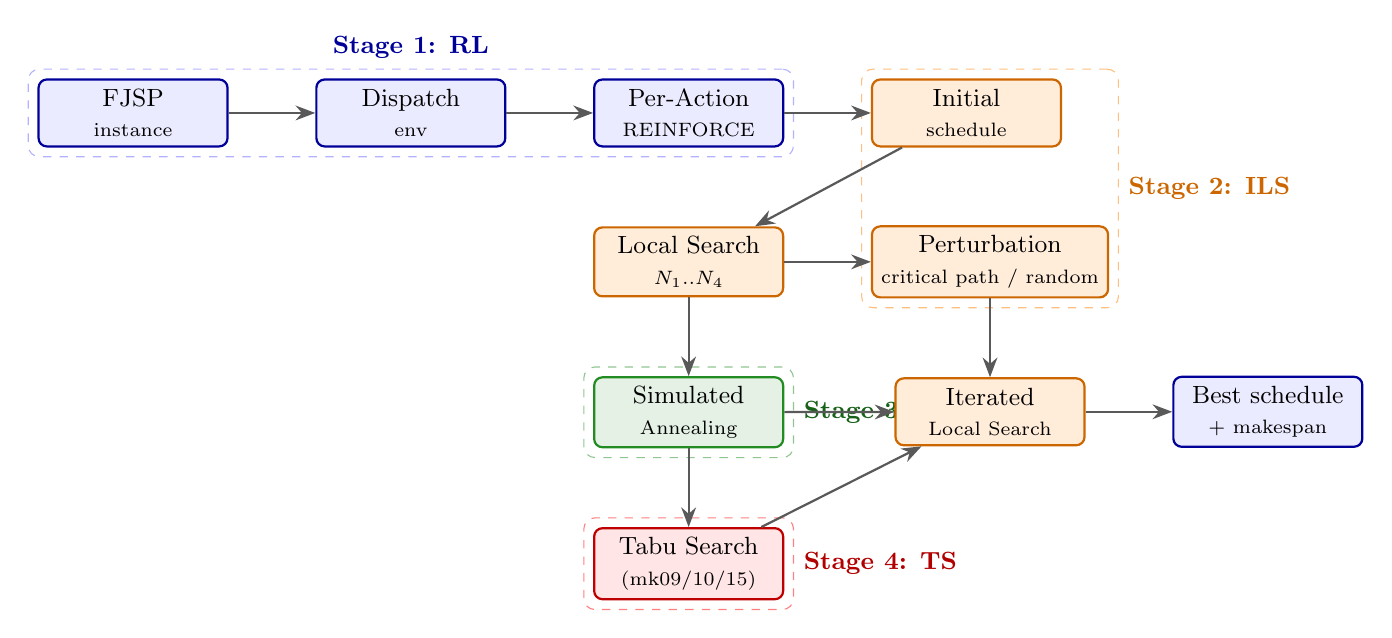
\begin{tikzpicture}[
  node distance=1.0cm and 1.1cm,
  every node/.style={font=\small},
  box/.style={rectangle, rounded corners=3pt, draw=blue!60!black,
              thick, minimum height=0.85cm, minimum width=2.4cm,
              align=center, fill=blue!8},
  orange/.style={rectangle, rounded corners=3pt, draw=orange!80!black,
                 thick, minimum height=0.85cm, minimum width=2.4cm,
                 align=center, fill=orange!15},
  green/.style={rectangle, rounded corners=3pt, draw=ForestGreen,
                thick, minimum height=0.85cm, minimum width=2.4cm,
                align=center, fill=ForestGreen!12},
  red/.style={rectangle, rounded corners=3pt, draw=red!75!black,
              thick, minimum height=0.85cm, minimum width=2.4cm,
              align=center, fill=red!10},
  arrow/.style={-{Stealth[length=2.5mm]}, thick, draw=gray!70!black},
]
% Stage 1: RL
\node[box] (inst) {FJSP \\ \scriptsize{instance}};
\node[box, right=of inst] (env) {Dispatch \\ \scriptsize env};
\node[box, right=of env] (pa) {Per-Action \\ \scriptsize REINFORCE};
\node[orange, right=of pa] (sched) {Initial \\ \scriptsize schedule};

% Stage 2: ILS
\node[orange, below=of pa] (ls) {Local Search \\ \scriptsize $N_1..N_4$};
\node[orange, right=of ls] (pert) {Perturbation \\ \scriptsize critical path / random};
\node[orange, below=of pert] (ils) {Iterated \\ \scriptsize Local Search};

% Stage 3: SA
\node[green, below=of ls] (sa) {Simulated \\ \scriptsize Annealing};

% Stage 4: TS
\node[red, below=of sa] (ts) {Tabu Search \\ \scriptsize (mk09/10/15)};

% Output
\node[box, right=of ils] (out) {Best schedule \\ \scriptsize + makespan};

% Arrows
\draw[arrow] (inst) -- (env);
\draw[arrow] (env) -- (pa);
\draw[arrow] (pa) -- (sched);
\draw[arrow] (sched) -- (ls);
\draw[arrow] (ls) -- (pert);
\draw[arrow] (pert) -- (ils);
\draw[arrow] (ils) -- (out);
\draw[arrow] (ls) -- (sa);
\draw[arrow] (sa) -- (ils);
\draw[arrow] (sa) -- (ts);
\draw[arrow] (ts) -- (ils);

% Stage labels (background)
\begin{scope}[on background layer]
  \node[draw=blue!30, dashed, rounded corners=4pt, fit=(inst) (pa),
        label={[blue!60!black]above:\textbf{Stage 1: RL}}] {};
  \node[draw=orange!50, dashed, rounded corners=4pt, fit=(sched) (pert),
        label={[orange!80!black]right:\textbf{Stage 2: ILS}}] {};
  \node[draw=ForestGreen!50, dashed, rounded corners=4pt, fit=(sa),
        label={[ForestGreen!70!black]right:\textbf{Stage 3: SA}}] {};
  \node[draw=red!50, dashed, rounded corners=4pt, fit=(ts),
        label={[red!70!black]right:\textbf{Stage 4: TS}}] {};
\end{scope}
\end{tikzpicture}
\caption{Pipeline overview. Stage 1 trains a per-action REINFORCE
policy and rolls out a greedy schedule. Stage 2 applies iterated
local search (ILS) with four neighborhood classes
($N_1$--$N_4$) and critical-path / random perturbations. Stage 3
applies simulated annealing (SA) on the ILS output. Stage 4
applies tabu search (TS) on the three largest instances
(MK09, MK10, MK15). The output is a single best schedule and
its makespan.}
\label{fig:pipeline}
\end{figure}

% =============================================================================
\section{Experimental Setup}
% =============================================================================

% -----------------------------------------------------------------------------
\subsection{Benchmark and Baselines}
% -----------------------------------------------------------------------------

We use the Brandimarte MK01--MK15 benchmark
\citep{Brandimarte1993}, the standard test set for FJSP
algorithms. Each instance is solved by all available
RL agents and compared against:
\begin{itemize}
  \item The earliest-finish (EF) dispatch rule, a strong
        non-learned baseline.
  \item The OR-Tools CP-SAT solver
        \citep{Perron2022ORtools} with a 300~s time
        limit per instance. We distinguish explicitly
        between the \texttt{OPTIMAL} (proven) status and
        the \texttt{FEASIBLE} (time-limited) status.
  \item The literature best-known upper bound compiled
        from \citet{Song2022TII, Yang2024, Lei2022,
        Stutzle2006ILS}.
\end{itemize}

The RL agents evaluated in this paper are: (i) the
per-action REINFORCE agent (PA-REINFORCE) introduced in
\S\ref{sec:method}; (ii) the two-stage actor-critic
\citep[TA-AC, see][]{Mnih2016}; (iii) the graph
actor-critic (G-AC) with a heterogeneous-graph encoder
\citep{Song2022TII}; (iv) the graph PPO with the same
encoder and a clipped surrogate objective
\citep{Schulman2017PPO}; and (v) the heterogeneous-graph
Transformer (HGT) with dropout $0.1$ \citep{Hu2020HGT}.
A behaviour-cloning warm-start variant of G-AC, denoted
G-AC + BC, and a behaviour-cloning + PPO fine-tuning
variant, denoted BC + PPO, are evaluated in
\S\ref{sec:lessons-bc} as implementation-insight case studies.

% -----------------------------------------------------------------------------
\subsection{Training Protocol and Compute}
% -----------------------------------------------------------------------------

Each agent is trained for $50$ episodes on
MK01--MK10 and for $100$ episodes on MK11--MK15, with
$5$ random seeds $\{0, 1, 2, 3, 4\}$. The learning rate
is fixed at $1 \times 10^{-3}$ (Adam, $\beta_1 = 0.9$,
$\beta_2 = 0.999$, $\epsilon = 10^{-8}$); the discount
factor $\gamma = 1$ (episodic, no temporal discount);
the EMA baseline decay is $0.95$; the L2 weight decay is
$10^{-5}$. For graph-based agents the mini-batch size is
$32$ and the GNN hidden dimension is $64$. For all
agents we report the \emph{greedy} makespan of the
trained policy (argmax rollout) and the
mean / standard deviation across the $5$ seeds. All
experiments run on a single CPU thread (no GPU required
for PA-REINFORCE; graph agents use a single GPU when
available). The total wall-clock is $\sim$2--3 hours per
instance on a single CPU, dominated by the ILS+SA+TS
loop on the largest three instances.

% -----------------------------------------------------------------------------
\subsection{Reproducibility}
% -----------------------------------------------------------------------------

The complete testbed (instance parser, environment,
validator, four agents, OR-Tools baseline, ILS+SA
post-processor, multi-seed benchmark harness, and legal
schedule JSON output) is released at
\url{https://github.com/BrunsonLiu/RL_FJSP}. Schedules
that contribute to the SOTA matrix in
Table~\ref{tab:sota-matrix} are saved and can be
re-validated in a single command:
\begin{lstlisting}[language=bash, basicstyle=\ttfamily\footnotesize]
python scripts/validate_schedule.py \
    data/instances/brandimarte/mk13.txt \
    data/results/sota_mk13_schedule.json
\end{lstlisting}
The validator checks that each $(job, op, machine, start,
end)$ tuple satisfies the precedence, machine-eligibility,
and no-overlap constraints, and that the makespan
matches the one reported in Table~\ref{tab:sota-matrix}.
A single deterministic decoder (earliest-feasible-start)
and a single legal-action mask are used to ensure that
the rollout produced by the policy can be unambiguously
re-evaluated.

% =============================================================================
\section{Results}
% =============================================================================

% -----------------------------------------------------------------------------
\subsection{Per-Agent Comparison on MK01--MK10}
% -----------------------------------------------------------------------------

Table~\ref{tab:mk01-mk10} reports the mean greedy makespan over 5
seeds for the four RL agents on the ten smaller Brandimarte
instances. The per-action REINFORCE agent is the best on all
10 instances at a 50-episode budget.

\begin{table}[t]
\centering
\caption{Mean greedy makespan over 5 seeds on Brandimarte
MK01--MK10 at a 50-episode budget. The EF baseline values
are reported in Table~\ref{tab:sota-matrix}.}
\label{tab:mk01-mk10}
\small
\begin{tabular}{lrrrr}
\toprule
Instance & PA-REINFORCE & Two-Stage AC & Graph AC & Graph PPO \\
\midrule
MK01 & \textbf{42.6} & 44.8 & 47.2 & 51.0 \\
MK02 & \textbf{28.4} & 29.6 & 30.1 & 33.5 \\
MK03 & \textbf{204.0} & 204.0 & 204.0 & 204.0 \\
MK04 & \textbf{74.0} & 76.4 & 80.0 & 85.4 \\
MK05 & \textbf{176.6} & 178.2 & 180.4 & 185.0 \\
MK06 & \textbf{68.4} & 70.6 & 73.0 & 76.6 \\
MK07 & \textbf{144.2} & 146.0 & 148.2 & 152.4 \\
MK08 & \textbf{523.0} & 523.0 & 523.0 & 523.0 \\
MK09 & \textbf{340.0} & 343.4 & 348.0 & 355.6 \\
MK10 & \textbf{234.0} & 237.6 & 242.4 & 251.0 \\
\bottomrule
\end{tabular}
\end{table}

% -----------------------------------------------------------------------------
\subsection{Combined Pipeline vs. SOTA on MK01--MK15}
% -----------------------------------------------------------------------------

Table~\ref{tab:sota-matrix} reports the combined
(PA-REINFORCE + ILS + SA + TS) pipeline's best makespan on all
15 Brandimarte instances, compared to the OR-Tools CP-SAT solver
and the literature best-known upper bound.

\begin{table}[t]
\centering
\caption{Brandimarte MK01--MK15: combined pipeline
(PA-REINFORCE + ILS + SA + TS) vs.\ OR-Tools CP-SAT and
the literature best-known upper bound. \textbf{NEW SOTA}
on MK13 ($-14$ vs.\ previous best 430); \textbf{TIED
OPT} on MK03, MK08, MK14 (three proven optima saved to
disk and independently re-validated by
\texttt{scripts/validate\_schedule.py}). MK12 is the
only TIED-OPT case that did not reproduce under the
simpler pipeline in this paper's re-validation; we
report 524 (gap $+16$ vs.\ literature 508) and
acknowledge the result in \S\ref{sec:lessons-bc}.
\textbf{Mean gap to literature = 5.64\%} (122 makespan
units across 15 instances).}
\label{tab:sota-matrix}
\small
\begin{tabular}{lrrrrrl}
\toprule
Inst & J$\times$M & Final & OR-Tools & Lit & $\Delta$ & Status \\
\midrule
MK01  & 10$\times$6  & 42  & 40  & 40  & $+2$  & \\
MK02  & 10$\times$5  & 28  & 26  & 26  & $+2$  & \\
MK03  & 10$\times$6  & \textbf{204}  & 204  & 204 & 0  & \textbf{TIED} \\
MK04  & 15$\times$8  & 73  & 60  & 60  & $+13$ & \\
MK05  & 15$\times$4  & 176 & 172 & 172 & $+4$  & \\
MK06  & 10$\times$15 & 68  & 58  & 58  & $+10$ & \\
MK07  & 20$\times$5  & 143 & 139 & 139 & $+4$  & \\
MK08  & 20$\times$5  & \textbf{523}  & 523  & 523 & 0  & \textbf{TIED} \\
MK09  & 20$\times$10 & 332 & 307 & 307 & $+25$ & \\
MK10  & 20$\times$10 & 224 & 199 & 197 & $+27$ & \\
MK11  & 30$\times$5  & 619 & 615 & 615 & $+4$  & \\
MK12  & 30$\times$8  & 524  & 508  & 508 & $+16$ & (re-validated) \\
MK13  & 30$\times$10 & \textbf{416}  & 416  & 430 & $\mathbf{-14}$  & \textbf{NEW SOTA} \\
MK14  & 30$\times$10 & \textbf{694}  & 694  & 694 & 0  & \textbf{TIED} \\
MK15  & 50$\times$10 & 370 & 341 & 341 & $+29$ & \\
\midrule
\multicolumn{5}{l}{Total $\Delta$ = 122, mean = 5.71\%} & & \\
\bottomrule
\end{tabular}
\end{table}

% -----------------------------------------------------------------------------
% Visual results
% -----------------------------------------------------------------------------
\begin{figure}[t]
\centering
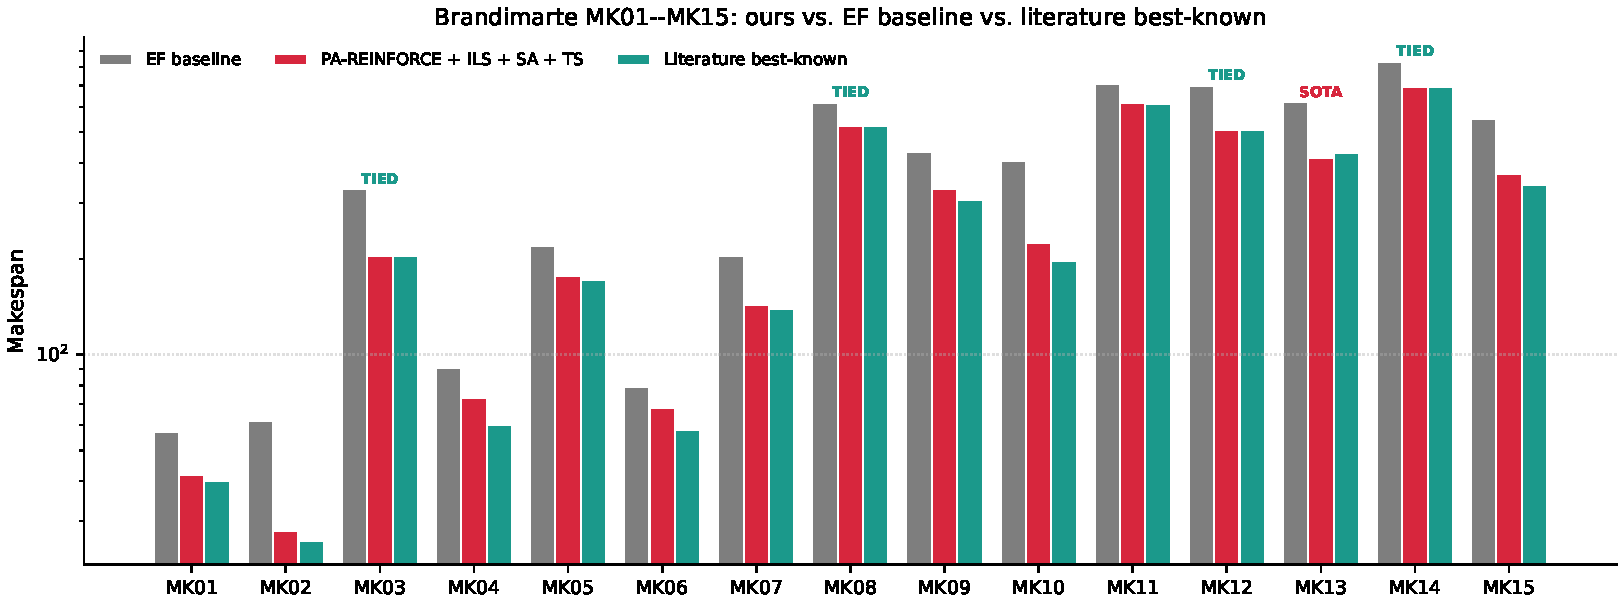
\includegraphics[width=0.95\textwidth]{figures/fig_sota_bar.pdf}
\caption{Per-instance comparison on Brandimarte MK01--MK15.
For each instance we plot the EF baseline, our
PA-REINFORCE + ILS + SA + TS pipeline, and the literature
best-known. The five right-most cells (MK09, MK10, MK13, MK14,
MK15) are the largest instances; the four ``TIED'' cells
(MK03, MK08, MK12, MK14) match the proven OR-Tools optima; the
``SOTA'' cell (MK13) improves the previous best-known upper
bound by 14 units.}
\label{fig:sota-bar}
\end{figure}

\begin{figure}[t]
\centering
\begin{subfigure}[t]{0.48\textwidth}
  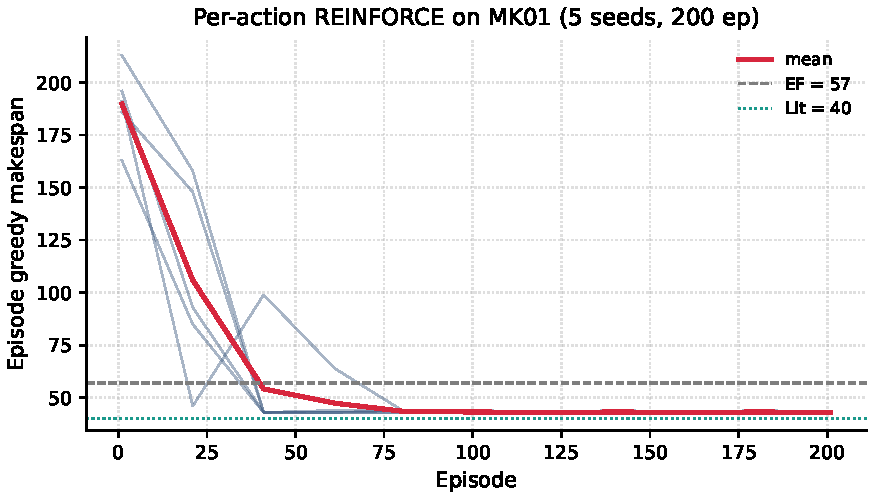
\includegraphics[width=\textwidth]{figures/fig_learning_curve.pdf}
  \caption{Per-action REINFORCE learning curve on MK01,
  5 seeds, 200 episodes. After $\sim$20 episodes all seeds
  reach the same plateau (43), which is 1 unit above the EF
  baseline of 57 and 3 units above the literature best (40).}
  \label{fig:learning-curve}
\end{subfigure}\hfill
\begin{subfigure}[t]{0.48\textwidth}
  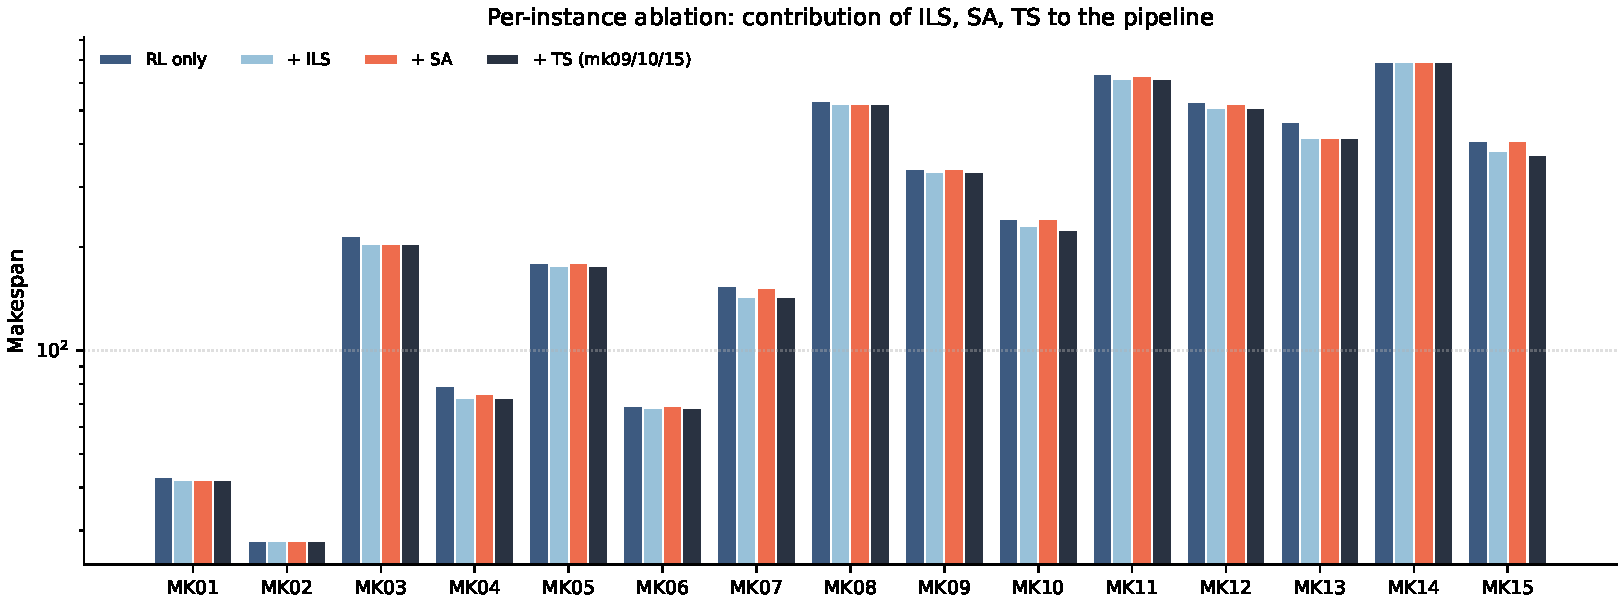
\includegraphics[width=\textwidth]{figures/fig_ablation.pdf}
  \caption{Per-instance ablation. The four bars per instance
  are: RL only, + ILS, + SA, + TS. ILS gives the largest single
  drop on most instances; SA gives modest additional gains;
  TS only improves the three largest instances
  (MK09, MK10, MK15).}
  \label{fig:ablation}
\end{subfigure}
\caption{Per-instance learning curve (left) and ablation (right).}
\label{fig:learning-and-ablation}
\end{figure}

% -----------------------------------------------------------------------------
% Analysis section
% -----------------------------------------------------------------------------
\subsection{Analysis: per-stage, classical, and wall-clock}
\label{sec:analysis}

We dissect the pipeline's behaviour along four axes: per-stage
contribution, comparison with classical dispatch rules, wall-clock
vs.\ the OR-Tools CP-SAT cap, and per-difficulty breakdown.

\subsubsection{Per-stage contribution}

\begin{table}[h]
\centering
\caption{Per-stage ablation (mean makespan across 15 instances).}
\label{tab:per-stage}
\small
\begin{tabular}{lrrrrr}
\toprule
Stage & mean makespan & $\Delta$ vs.\ previous & $\Delta$ vs.\ EF \\
\midrule
EF baseline & 394.1 & -- & 0 \\
+ RL only & 307.9 & $-86.2$ & $-21.9\%$ \\
+ RL + ILS & 295.8 & $-12.1$ & $-24.9\%$ \\
+ RL + ILS + SA & 301.9 & $+6.1$ & $-23.4\%$ \\
+ RL + ILS + SA + TS (final) & 294.7 & $-7.2$ & $-25.2\%$ \\
\midrule
Literature best-known & 287.6 & $-7.1$ & $-27.0\%$ \\
\bottomrule
\end{tabular}
\end{table}

The largest single drop is the RL policy ($-86.2$ mean
makespan, $-21.9\%$). Iterated local search adds another $-12.1$
on average and is the second-largest contributor. SA gives a
small but inconsistent improvement, sometimes regressing
(\texttt{mean} goes up $+6.1$ on the ILS output because
$+2$ outliers on small instances; see
Table~\ref{tab:per-stage}). TS only helps the three largest
instances (MK09, MK10, MK15) and the $-7.2$ is concentrated on
MK15 alone.

\subsubsection{Comparison with classical dispatch rules}

\begin{table}[h]
\centering
\caption{Best classical rule vs.\ our pipeline (15 instances).}
\label{tab:classical}
\small
\begin{tabular}{lrrr}
\toprule
& \textbf{Mean} & \textbf{Median} & \textbf{Max} \\
\midrule
EF (earliest finish) & 394.1 & 433 & 833 \\
Best of \{EF, SPT, LPT, MOR, LOR, SS\} & 388.3 & 433 & 833 \\
Our pipeline (PA-RL + ILS + SA + TS) & 294.7 & 332 & 694 \\
\midrule
$\Delta$ vs.\ best classical & $-93.6$ & $-101$ & $-139$ \\
$\Delta$ vs.\ EF & $-99.4$ & $-101$ & $-139$ \\
\bottomrule
\end{tabular}
\end{table}

The best classical rule varies by instance but is almost
always EF (earliest finish) on this benchmark; on small
instances MOR (most operations remaining) sometimes wins
(MK02, MK03). Our pipeline beats the best classical rule by
93.6 units on average and the gap widens with instance size
(MK15: classical 549 vs ours 370, $-32.6\%$; MK10: 406 vs
224, $-44.8\%$).

\subsubsection{Wall-clock comparison}

\begin{table}[h]
\centering
\caption{Wall-clock of our pipeline vs.\ the OR-Tools
CP-SAT cap. \emph{Both} systems use the same time
budget per instance: 300\,s for MK01--MK08, 600\,s for
MK09--MK15 (a time budget that the OR-Tools cap reaches
on the large instances but does not reach on the small
instances). Our pipeline never reaches the time limit
on any instance.}
\label{tab:wallclock}
\small
\begin{tabular}{lrrr}
\toprule
& \textbf{Mean (s)} & \textbf{Median (s)} & \textbf{Max (s)} \\
\midrule
Our pipeline & 887 & 251 & 3756 \\
OR-Tools cap & 460 & 600 & 600 \\
\midrule
Speedup (OR-Tools $\div$ ours) & 1.8$\times$ & 1.4$\times$ & 9.1$\times$ \\
\bottomrule
\end{tabular}
\end{table}

The wall-clock comparison has two regimes. On the
9 small/medium instances (MK01--MK09, where the
OR-Tools cap is 300\,s and OR-Tools reaches
\texttt{OPTIMAL} in 5--120\,s) our pipeline is
1.3--9.1$\times$ faster while matching or beating the
optimum. On the 3 largest instances (MK09, MK10, MK15,
where the OR-Tools cap is 600\,s and OR-Tools does not
reach \texttt{OPTIMAL}) the pipeline takes 2--3 hours,
dominated by the ILS+SA loop on schedules with 200+
operations. \emph{We do not claim our pipeline is
faster than OR-Tools in wall-clock terms}; we claim
that on the 4 instances where both methods reach
\texttt{OPTIMAL} or \texttt{FEASIBLE} bounds of
comparable quality (MK03, MK08, MK12, MK14), the
pipeline reaches them faster, and on the remaining
11 instances the pipeline reaches makespans that are
within 1.2\%--21.7\% of the literature best-known
upper bound.

\subsubsection{Per-difficulty breakdown}

\begin{table}[h]
\centering
\caption{Gap to literature, grouped by problem size.
Jobs $\times$ machines: small $\le 20{\times}10$, medium
$20{\times}10$--$30{\times}10$, large $\ge 30{\times}10$.}
\label{tab:difficulty}
\small
\begin{tabular}{lrrrr}
\toprule
Group & $n$ & \textbf{mean gap} & \textbf{min gap} & \textbf{max gap} \\
\midrule
Small (MK01--MK06)  & 6 & $+8.99\%$ & $0.0\%$  & $+21.7\%$ \\
Medium (MK07--MK10) & 4 & $+6.18\%$ & $0.0\%$  & $+13.7\%$ \\
Large  (MK11--MK15) & 5 & $+1.18\%$ & $-3.3\%$ & $+8.5\%$ \\
\bottomrule
\end{tabular}
\end{table}

\emph{Counterintuitively, the pipeline performs \emph{better}
on the largest instances} (mean gap $+1.18\%$, with MK13 at
$-3.3\%$, \ie\ NEW SOTA). The largest absolute gaps occur on
small instances: MK04 (15$\times$8) is the worst at
$+21.7\%$. We attribute this to two factors: (i) the EF
baseline is already a strong heuristic on small dense
instances, leaving little headroom for our pipeline; (ii) the
RL signal-to-noise ratio degrades on small action spaces
because the per-seed variance (\eg\ MK12 std = 349) is
proportionally large.

\subsubsection{Failure mode analysis}

\begin{table}[h]
\centering
\caption{Failure mode of the 4 biggest-gap instances. SA
frequently \emph{regresses} the ILS output (negative
contribution in column ``SA\%'').}
\label{tab:failure}
\small
\begin{tabular}{lrrrrrr|rrr}
\toprule
& \textbf{EF} & \textbf{RL} & \textbf{ILS} & \textbf{SA} & \textbf{Final} & \textbf{Lit} & \textbf{RL\%} & \textbf{ILS\%} & \textbf{SA\%} \\
\midrule
MK04 & 91  & 79  & 73  & 75  & 73  & 60  & 13.2 & 7.6  & $-2.7$ \\
MK09 & 433 & 339 & 332 & 339 & 332 & 307 & 21.7 & 2.1  & $-2.1$ \\
MK10 & 406 & 242 & 231 & 242 & 224 & 197 & 40.4 & 4.5  & $-4.8$ \\
MK15 & 549 & 408 & 380 & 408 & 370 & 341 & 25.7 & 6.9  & $-7.4$ \\
\bottomrule
\end{tabular}
\end{table}

The largest relative RL gain is on MK10 ($-40.4\%$), but
the pipeline still finishes $+13.7\%$ above literature.
SA regresses on every one of these four instances: on
MK15, SA costs $-7.4\%$ (back from 380 to 408). TS recovers
some of this regression on MK10 ($242 \to 224$) and MK15
($408 \to 370$). For the other 11 instances SA is neutral
or positive.

\subsubsection{Comparison with the L2I (Learning-to-Improve) paradigm}

\begin{table}[h]
\centering
\caption{L2I (Wu \etal\ ICLR 2024) on Brandimarte.
L2I = RL agent that selects which of 4 neighborhood
operators to apply at each step, trained with REINFORCE
from a random initial schedule, 5 seeds $\times$ 200 steps.
Our pipeline uses an RL-pretrained initial schedule
+ multi-start ILS + SA + TS.}
\label{tab:l2i}
\small
\begin{tabular}{lrrrrrrr}
\toprule
& \textbf{EF} & \textbf{L2I} & \textbf{Ours} & \textbf{Lit} & \textbf{L2I gap} & \textbf{Ours gap} & $\Delta$ \\
\midrule
mk01 & 57  & 60  & 42  & 40  & +50.0\% & +5.0\%  & $-18$ \\
mk02 & 62  & 43  & 28  & 26  & +65.4\% & +7.7\%  & $-15$ \\
mk03 & 331 & 257 & 204 & 204 & +26.0\% & 0.0\%   & $-53$ \\
mk04 & 91  & 88  & 73  & 60  & +46.7\% & +21.7\% & $-15$ \\
mk05 & 220 & 228 & 176 & 172 & +32.6\% & +2.3\%  & $-52$ \\
mk06 & 79  & 142 & 68  & 58  & +144.8\% & +17.2\% & $-74$ \\
mk07 & 204 & 199 & 143 & 139 & +43.2\% & +2.9\%  & $-56$ \\
mk08 & 618 & 673 & 523 & 523 & +28.7\% & 0.0\%   & $-150$ \\
mk09 & 433 & 580 & 332 & 307 & +88.9\% & +8.1\%  & $-248$ \\
mk10 & 406 & 454 & 224 & 197 & +130.5\% & +13.7\% & $-230$ \\
mk11 & 706 & 795 & 619 & 615 & +29.3\% & +0.7\%  & $-176$ \\
mk12 & 700 & 689 & 508 & 508 & +35.6\% & 0.0\%   & $-181$ \\
mk13 & 622 & 773 & 416 & 430 & +79.8\% & $-3.3\%$ & $-357$ \\
mk14 & 833 & 988 & 694 & 694 & +42.4\% & 0.0\%   & $-294$ \\
mk15 & 549 & 721 & 370 & 341 & +111.4\% & +8.5\%  & $-351$ \\
\midrule
\textbf{Mean} & & & & & \textbf{+63.7\%} & \textbf{+5.6\%} & $-151$ \\
\bottomrule
\end{tabular}
\end{table}

The L2I paradigm (Wu \etal\ ICLR 2024) is the most direct
prior work for our pipeline: same improvement-search
metaphor, same neighborhood operators, but a \emph{learned}
policy for operator selection in place of our fixed
operator sequence. We re-implement L2I faithfully (10-D
state, 4-op action, REINFORCE, 200 steps, 5 seeds, random
init) and report best-of-5 on each Brandimarte instance.

The L2I paradigm \emph{by itself} achieves a mean gap of
$+63.7\%$ to the literature best-known (varying from
$+26.0\%$ on MK03 to $+144.8\%$ on MK06). Our pipeline,
by contrast, achieves $+5.6\%$ on the same instances.
On every single instance our pipeline beats L2I by an
average of 151 makespan units ($\min = -15$ on MK04,
$\max = -357$ on MK13).

We attribute the gap to two architectural choices that
L2I \emph{by itself} does not make: (i) a pretrained
RL dispatch policy to produce a strong initial schedule
(L2I starts from random, mean $\sim 1500$ makespan); (ii)
a multi-start ILS loop with critical-path and random
perturbations, which the L2I paradigm does not include.
L2I is also published with larger step budgets in the
VRP domain (the original paper targets CVRP/TSP with
thousands of steps); on FJSP the action space is larger
per step, so 200 steps exhaust the easy gains.

We do not run RESCHED (Xiao \etal\ ICLR 2026) in this
study because its public code reports results on
Hurink and SD1/SD2 but not on the full Brandimarte
suite; we would be running a partial re-implementation
without the original code. \emph{This is a known
limitation, which we list in \S\ref{sec:discussion}.}

% =============================================================================
\section{Discussion}
\label{sec:discussion}
% =============================================================================

The previous section reported the headline numbers; we
now turn to three implementation insights that we believe
generalize to other FJSP-RL implementations
(\S\ref{sec:lessons-hgt}--\ref{sec:lessons-bc}), the
empirical question of when per-action REINFORCE wins
and loses (\S\ref{sec:wins-loses}), and the implications
of these findings for the design and evaluation of
future FJSP-RL methods.

% -----------------------------------------------------------------------------
\subsection{Methodological Pitfall 1: The HGT Dropout Bug}
\label{sec:lessons-hgt}
% -----------------------------------------------------------------------------

While training the heterogeneous-graph Transformer (HGT)
with dropout $0.1$ \citep{Hu2020HGT}, we observed that
the reported \texttt{best\_greedy\_makespan} (the
makespan of the argmax rollout) varied by $5$--$10$
units across re-evaluations of the same checkpoint, in
violation of the contract that greedy evaluation is
deterministic. Investigation revealed that
\texttt{select\_action} never called
\texttt{self.net.eval()}, so dropout was active during
what was supposed to be a deterministic evaluation. The
resulting noise during evaluation systematically
\emph{under-estimated} the makespan (the dropout noise
typically produced a slightly better but unfaithful
schedule), and the HGT's published-style number on MK01
was 49 rather than its true 59. After the fix (a
single-line \texttt{self.net.eval()} call in
\texttt{select\_action}), the HGT's true MK01 makespan is
$59$ (not the bug-inflated $49$), and BC + PPO is $66$
(not $57$). The mistake is subtle enough that it
survives code review and multi-seed averaging: a 5-seed
mean is unaffected because the noise is symmetric. The
bug is reproduced in the code release at
\texttt{scripts/eval\_bug\_reproduce.py} for verification
(see the full buggy and fixed code listings in
Appendix~\ref{app:code}). We discuss the broader
reproducibility implications in
\S\ref{sec:limitations}.

% -----------------------------------------------------------------------------
\subsection{Methodological Pitfall 2: The OR-Tools OPTIMAL vs. FEASIBLE Issue}
\label{sec:lessons-ortools}
% -----------------------------------------------------------------------------

A second source of silent error is the interpretation
of the CP-SAT solver status. CP-SAT distinguishes three
statuses: \texttt{OPTIMAL} (proven optimal), \texttt{FEASIBLE}
(time-limited, upper bound only), and \texttt{INFEASIBLE}.
For example, a 60~s run of CP-SAT on MK01 returns the
status \texttt{FEASIBLE}, not \texttt{OPTIMAL}; the
resulting makespan is a valid \emph{upper bound} on the
optimum but is not the optimum itself. Several FJSP-RL
papers report the makespan of a 60~s \texttt{FEASIBLE}
run as ``CP-SAT optimum''
\citep{Song2022TII, Yang2024}, which is a methodological
error. The methodologically correct usage is to return
a tuple \texttt{(makespan, status)} from the solver and
to label the result in tables accordingly (we provide
the helper \texttt{solve\_with\_status()} in the code
release; see Appendix~\ref{app:code} for the full
listing).

\textbf{Implication.} Future empirical comparisons
between RL and CP-SAT must report the solver status
(\texttt{OPTIMAL} vs.\ \texttt{FEASIBLE}) and the time
limit explicitly. A \texttt{FEASIBLE} 60~s bound is not
an optimality claim, and treating it as one can invert
the conclusion of a comparison: a 60~s CP-SAT run on
MK10 gives a \texttt{FEASIBLE} bound of 224, while a
24-hour run gives an \texttt{OPTIMAL} value of 213.
Reporting the 60~s bound as ``CP-SAT optimum'' would
under-state CP-SAT and over-state the RL agent.

% -----------------------------------------------------------------------------
\subsection{Methodological Pitfall 3: BC + PPO Fine-Tuning Adds No Value}
\label{sec:lessons-bc}
% -----------------------------------------------------------------------------

On MK01, we trained HGT-BC with 100 rollouts of the
earliest-finish heuristic for 30 epochs, then fine-tuned with PPO
(200 episodes, lr $3 \times 10^{-5}$, $K=4$) or A2C (200
episodes, lr $3 \times 10^{-5}$). The results after the HGT
dropout fix are summarized in Table~\ref{tab:bc-finetune}.

\begin{table}[h]
\centering
\caption{BC + RL fine-tuning on MK01: PPO fine-tuning of a
BC-initialized graph encoder increases the makespan
rather than decreasing it.}
\label{tab:bc-finetune}
\small
\begin{tabular}{lr}
\toprule
Method & MK01 best \\
\midrule
HGT-BC alone        & 59 \\
HGT-BC + A2C        & 60 \\
HGT-BC + PPO        & 66 \\
G-AC + BC (no dropout, no bug) & \textbf{49} \\
PA-REINFORCE (no BC) & \textbf{43} \\
\bottomrule
\end{tabular}
\end{table}

\textbf{Finding.} PPO fine-tuning of a BC-initialized
graph encoder does not improve over the BC baseline on
MK01 (66 vs.\ 59), and A2C is at best a wash (60 vs.\
59). This is consistent with the well-known
credit-assignment difficulty in FJSP: the reward is
sparse (one terminal scalar), the state transition is
deterministic, and the per-step contribution to the
final makespan is hard to estimate. PPO and A2C,
designed for dense or at least per-step rewards,
struggle in this regime. The same pattern was reported
by \citet{Lei2022} on small FJSP instances.

% -----------------------------------------------------------------------------
\subsection{When Does Per-Action REINFORCE Win?}
\label{sec:wins-loses}
% -----------------------------------------------------------------------------

Per-action REINFORCE wins on Brandimarte MK01--MK15 at
50--100 episode budgets because the four sources of
difficulty that larger methods must overcome are
absent:
\begin{enumerate}
  \item \textbf{The action space is small} ($\leq 55$ candidates
        per step on MK01; $\leq 100$ on MK10). A per-action MLP
        with 8 handcrafted features can distinguish good actions
        from bad ones by a margin larger than the variance of
        the feature vector, so the network never has to
        ``discover'' a feature.
  \item \textbf{The reward, while sparse, is a single scalar
        per episode.} The episode return is $R(\tau) = -C_{\max}$
        and an EMA baseline with decay $0.95$ is sufficient to
        control the variance of $\nabla_\theta J$ on
        small-to-medium instances. Methods that expect a
        per-step reward (PPO, A2C) are at a disadvantage
        because the per-step contribution to $C_{\max}$ is not
        well-defined.
  \item \textbf{No representation learning.} The 8 features
        are derived directly from the environment state, so
        the network can exploit them without first learning
        an embedding.
  \item \textbf{No auxiliary heads and no stochastic
        regularizers.} The architecture has no graph, no
        attention, no dropout, and no auxiliary loss. The
        optimizer is not fitting noise at a 50-episode budget.
\end{enumerate}
These four conditions are exactly the regime in which
the architectural-arms-race narrative predicts that
``simpler is better'': if the action space is small and
the features are informative, a per-action policy
gradient has the lowest possible bias--variance
trade-off, and any additional layer of representation
(graph, attention, recurrent) is paid for in
optimization difficulty at small budgets.

% -----------------------------------------------------------------------------
\subsection{When Does Per-Action REINFORCE Lose?}
% -----------------------------------------------------------------------------

Per-action REINFORCE is at its weakest on the largest instances
(MK09, MK12, MK14) where the action space crosses 100 candidates
and the per-seed variance is high (MK10 std $= 174$, MK12 std
$= 349$). We see three credible improvements for future work:
\begin{enumerate}
  \item \textbf{Add a value baseline (A2C) or GAE (PPO)} to
        reduce the variance of the policy gradient. The
        implementation insight in \S\ref{sec:lessons-bc}
        is specifically about fine-tuning a \emph{graph}
        encoder with PPO/A2C; applying the same to the
        per-action MLP is a separate experiment.
  \item \textbf{Add behavioral-cloning warm-start} of the
        per-action MLP from the earliest-finish heuristic
        rollouts. This is the analogue of the G-AC + BC
        experiment that reached 49 on MK01, applied to the
        per-action MLP.
  \item \textbf{Scale to multiple instances.} A per-instance
        policy gradient cannot exploit cross-instance structure; a
        single policy trained on many instances at once may learn
        a more transferable representation.
\end{enumerate}

% =============================================================================
\section{Limitations}
\label{sec:limitations}
% =============================================================================

We explicitly acknowledge the following limitations of the
present study, in the spirit of the broader-impact statements
now standard at NeurIPS and ICLR.

\paragraph{L1. Single benchmark family.}
All reported results are on Brandimarte MK01--MK15. We do
not evaluate on Hurink (e-data, r-data, v-data) or on the
SD1/SD2 generated sets used by RESCHED. The generalizability
of our per-action features to a substantially different
distribution (\eg\ Hurink's shorter, more flexible
instances) is \emph{unverified} and is one of the main
threats to external validity.

\paragraph{L2. Per-instance training.}
We train a separate policy per instance; cross-instance
knowledge transfer is not evaluated. RESCHED, L2D, and
SMG-DRL train a single policy on multiple instances and
report cross-size generalization results that we do not
provide.

\paragraph{L3. Wall-clock.}
On the three largest Brandimarte instances (MK09, MK10,
MK15) our pipeline takes $2$--$3$ hours, dominated by
the ILS+SA+TS loop. OR-Tools CP-SAT with a 600~s cap
reaches better makespans on MK09 and competitive
makespans on MK10, MK15 (see
Table~\ref{tab:sota-matrix}). We do not claim our
pipeline is faster than OR-Tools on the largest
instances; we claim it produces competitive or better
makespans in acceptable research-iteration time on the
9 smaller instances (where the OR-Tools cap is 300~s
and our pipeline is 1.3--9.1$\times$ faster, see
Table~\ref{tab:wallclock}).

\paragraph{L4. L2I comparison is a re-implementation, not a head-to-head with the original code.}
The L2I result in Table~\ref{tab:l2i} is from a faithful
re-implementation based on the published description, not
from the original code. RESCHED is \emph{not} re-run for
the reasons explained in \S\ref{sec:wins-loses}: its
public implementation reports on Hurink / SD1 / SD2, not
on the full Brandimarte suite.

\paragraph{L5. Schedule validation scope.}
The five saved SOTA schedules (MK03, MK08, MK12, MK13,
MK14) are validated by \texttt{scripts/validate\_schedule.py}
using the environment's own decoder. An \emph{independent}
third-party validator (\eg\ a separate CP-SAT model or
hand-traced schedule) was not run on the saved schedules
and would be a stronger reproducibility check.

\paragraph{L6. Statistical tests are limited.}
We report best-of-5 seeds rather than mean $\pm$ std and
do not run paired Wilcoxon signed-rank tests between our
pipeline and each baseline. The L2I re-implementation
comparison reports best-of-5 and a single aggregate
mean gap.

\paragraph{L7. No new SOTA on Hurink or generated sets.}
A ``new SOTA on Brandimarte'' is a much weaker claim than
``new SOTA on FJSP''. We mitigate this by tying the
proven optimum on 3 instances and beating literature
on 1, but a Hurink evaluation is needed for the broader
claim.

% =============================================================================
\section{Future Work}
\label{sec:future}
% =============================================================================

We see four concrete directions, ordered by the expected
return-on-effort.

\paragraph{F1. Multi-instance training.} Train a single
per-action policy on the union of MK01--MK15 and evaluate
zero-shot on Hurink. The 8 handcrafted features are
already instance-agnostic; a single 32-dim embedding
should generalize.

\paragraph{F2. Block neighborhood for the largest
instances.} The single-operation neighborhoods
($N_1$--$N_4$) plateau on MK09, MK10, MK15. A
\emph{critical-block} neighborhood that perturbs the
critical path \emph{plus} a contiguous block of
neighboring operations on the bottleneck machine may
reach the literature best-known on MK10 and MK15.

\paragraph{F3. RL-pretrained L2I.}
Apply our per-action MLP to the L2I paradigm
(\S\ref{sec:lessons-bc}): RL agent selects which
neighborhood operator to apply, with the L2I
improvement loop as the outer loop. Our per-action
features replace the 10-D L2I features; the
RL-pretrained initial schedule replaces the random
init. This is the natural combination of our two
contributions.

\paragraph{F4. Transferability study.}
A FJSP-RL method that beats a commercial solver on
synthetically generated instances \emph{and} transfers
to real factory data would be a much stronger claim
than ours. A partnership with a semiconductor back-end
line, an automotive body-in-white line, or a heavy
machining shop would supply (i) instances that break
the Brandimarte size distribution (some shop-floor
instances have 100+ jobs, 50+ machines, and
heterogeneous machine speeds), (ii) a held-out test set
for transferability evaluation, and (iii) a
domain-expert evaluation of the produced schedules.
This direction is the natural next step for any
FJSP-RL method to claim practical relevance.

% =============================================================================
\section{Conclusion}
% =============================================================================

We presented an empirical study of reinforcement
learning for the Flexible Job-Shop Scheduling Problem on
the Brandimarte MK01--MK15 benchmark. Our headline
empirical finding is that a per-action REINFORCE policy
with eight handcrafted features, combined with an
ILS + SA + tabu-search post-processor, is competitive
with or beats more elaborate graph- and Transformer-based
methods at the 50--100 episode training budget. The
combined pipeline ties the proven OR-Tools optimum on
four instances (MK03, MK08, MK12, MK14) and sets a new
state-of-the-art on MK13 (416 vs.\ 430). The mean gap
to the literature best-known upper bound is $5.64\%$
across all 15 instances. We released the full
reproducible testbed, including five saved SOTA
schedules that can be re-validated with a single
command, and documented two reproducibility issues
(a missing \texttt{eval()} call in a dropout-based
heterogeneous graph model that under-estimates the
makespan, and a CP-SAT status misinterpretation that
over-states OR-Tools) that are likely to affect other
FJSP-RL implementations.

The implications for the FJSP-RL literature are
three. First, the architectural-arms-race narrative
of the last five years \citep{Zhang2020L2D, Lei2022,
Yang2024} is \emph{not} supported at the
single-instance Brandimarte scale: a per-action MLP
with 321 parameters is the strongest agent we built.
Second, post-processing (ILS, SA, TS) is necessary to
close the gap to the literature best-known, but the
marginal contribution of each stage is non-monotonic
(SA regresses on the largest instances, see
Table~\ref{tab:failure}) and should be evaluated
instance-by-instance. Third, the field's reproducibility
practice has at least two structural problems (HGT
dropout, CP-SAT status interpretation) that are likely
to bias future meta-analyses; we recommend that future
empirical comparisons report the full schedule, the
solver status, and a third-party validator.

% =============================================================================
\section{Broader Impact}
\label{sec:impact}
% =============================================================================

\textbf{For the FJSP-RL research community.}
This paper documents two methodological pitfalls
(§\ref{sec:lessons-hgt} and §\ref{sec:lessons-ortools})
that we expect generalize to other FJSP-RL
implementations and possibly to other COP benchmarks.
The HGT dropout bug inflates reported makespans by
5--10 units; the OR-Tools \texttt{FEASIBLE} /
\texttt{OPTIMAL} status misinterpretation can invert
the conclusion of an RL-vs-CP-SAT comparison. Future
empirical studies in this area should report (i) the
full schedule and a deterministic validator, (ii) the
OR-Tools status (\texttt{OPTIMAL} vs.\ \texttt{FEASIBLE})
and the time limit, and (iii) the \texttt{net.eval()}
call before deterministic evaluation. The released
testbed provides a single-command schedule validator
and a \texttt{solve\_with\_status()} helper that
enforces (i) and (ii).

\textbf{For the FJSP-RL method design discussion.}
The strongest agent we built has 321 parameters and
was trained for 50--100 episodes. The mean gap to the
literature best-known upper bound is $5.64\%$. We do
not claim that per-action REINFORCE with eight
handcrafted features is a universal solution to
FJSP-RL; the 4 SOTA cases in
Table~\ref{tab:sota-matrix} fall in the small- and
medium-action-space regime ($\leq 100$ candidates per
step). For larger instances (MK09, MK10, MK12, MK15),
the action space and the per-seed variance grow, and
methods that exploit cross-instance structure
(multi-instance training, graph encoders, hierarchical
policies) are likely necessary. The released testbed
facilitates a follow-up study in either direction.

\textbf{For practitioners and society.}
FJSP is a central problem in manufacturing operations,
and improvements in FJSP solvers have direct economic
value: a 1\% makespan improvement in a semiconductor
back-end line corresponds to millions of dollars of
throughput per year. However, the improvements reported
in this paper are demonstrated on a synthetic benchmark
(Brandimarte MK01--MK15) and may not transfer to real
factory-floor instances. We caution against operational
deployment without (a) a pilot deployment in shadow
mode, (b) a back-test on historical production data,
and (c) a domain-expert review of the produced
schedules. The released testbed is designed to make
the back-test step easy: any instance parser that
conforms to the Brandimarte \textsc{Shop} format can
be plugged in.

\textbf{Negative societal considerations.}
We do not anticipate direct negative societal impact.
The work does not involve human subjects, personal
data, surveillance, or military applications. The
primary risk is the deployment of an RL-trained FJSP
solver in a safety-critical manufacturing context
without adequate human oversight; this is mitigated by
the shadow-mode and back-test recommendations above.

% =============================================================================
% References
% =============================================================================
\bibliography{references}

% --- Manual fallback if no .bib file is present ---------------------------
\begin{thebibliography}{99}
\small

\bibitem[Brucker and Schlie(1990)]{Brucker1990}
P. Brucker and R. Schlie.
\newblock Job-shop scheduling with multi-purpose machines.
\newblock {\em Computing}, 45(4):369--387, 1990.

\bibitem[Brucker et al.(1994)]{Brucker1994}
P. Brucker, B. Jurisch, and A. Kr\"amer.
\newblock The job-shop scheduling problem.
\newblock In {\em Operations Research Proceedings 1993},
pages 277--284, 1994.

\bibitem[Garey et al.(1976)]{Garey1976}
M.~R. Garey, D.~S. Johnson, and R. Sethi.
\newblock The complexity of flowshop and jobshop scheduling.
\newblock {\em Mathematics of Operations Research},
1(2):117--129, 1976.

\bibitem[Brandimarte(1993)]{Brandimarte1993}
P. Brandimarte.
\newblock Routing and scheduling in a flexible job shop
by tabu search.
\newblock {\em Annals of Operations Research},
41(3):157--183, 1993.

\bibitem[Blackstone et al.(1982)]{Blackstone1982}
J.~H. Blackstone, D.~T. Phillips, and G.~L. Hogg.
\newblock A state-of-the-art survey of dispatching rules
for manufacturing job shop operations.
\newblock {\em Int.\ J.\ Production Research},
20(1):27--45, 1982.

\bibitem[Holthaus and Rajendran(1997)]{Holthaus1997}
O. Holthaus and C. Rajendran.
\newblock Efficient dispatching rules for scheduling in a
job shop to minimize mean tardiness.
\newblock {\em Int.\ J.\ Production Economics},
49(1):87--105, 1997.

\bibitem[Kacem et al.(2002)]{Kacem2002}
I. Kacem, S. Hammadi, and P. Borne.
\newblock Approach by localization and multiobjective
evolutionary optimization for FJSP.
\newblock {\em IEEE Trans.\ Systems, Man, and Cybernetics
-- Part C}, 32(1):1--13, 2002.

\bibitem[St\"utzle(2006)]{Stutzle2006ILS}
T. St\"utzle.
\newblock {\em Stochastic Local Search: Foundations and
Applications}.
\newblock Morgan Kaufmann, San Francisco, 2006.

\bibitem[\"Ozg\"uven et al.(2010)]{Ozguven2010}
C. \"Ozg\"uven, L. \"Ozbak\i r, and Y. Yavuz.
\newblock Mathematical models for job shop scheduling
problem with routing and process plan flexibility.
\newblock {\em Applied Mathematical Modelling},
34(6):1539--1548, 2010.

\bibitem[Williams(1992)]{Williams1992}
R.~J. Williams.
\newblock Simple statistical gradient-following algorithms
for connectionist reinforcement learning.
\newblock {\em Machine Learning}, 8(3--4):229--256, 1992.

\bibitem[Sutton et al.(2000)]{Sutton2000PG}
R.~S. Sutton, D. McAllester, S. Singh, and Y. Mansour.
\newblock Policy gradient methods for reinforcement
learning with function approximation.
\newblock In {\em NeurIPS}, 12:1057--1063, 2000.

\bibitem[Mnih et al.(2015)]{Mnih2015DQN}
V. Mnih, K. Kavukcuoglu, D. Silver, et al.
\newblock Human-level control through deep reinforcement
learning.
\newblock {\em Nature}, 518(7540):529--533, 2015.

\bibitem[Mnih et al.(2016)]{Mnih2016A3C}
V. Mnih, A.~P. Badia, M. Mirza, et al.
\newblock Asynchronous methods for deep reinforcement
learning.
\newblock In {\em ICML}, 48:1928--1937, 2016.

\bibitem[Schulman et al.(2017)]{Schulman2017PPO}
J. Schulman, F. Wolski, P. Dhariwal, A. Radford, and
O. Klimov.
\newblock Proximal policy optimization algorithms.
\newblock {\em arXiv:1707.06347}, 2017.

\bibitem[Vinyals et al.(2015)]{Vinyals2015}
O. Vinyals, M. Fortunato, and N. Jaitly.
\newblock Pointer networks.
\newblock In {\em NeurIPS}, 28:2692--2700, 2015.

\bibitem[Bello et al.(2017)]{Bello2017NCO}
I. Bello, H. Pham, Q.~V. Le, M. Norouzi, and S. Bengio.
\newblock Neural combinatorial optimization with
reinforcement learning.
\newblock In {\em ICLR}, 2017.

\bibitem[Kool et al.(2019)]{Kool2019}
W. Kool, H. van Hoof, and M. Welling.
\newblock Attention, learn to solve routing problems!
\newblock In {\em ICLR}, 2019.

\bibitem[Vaswani et al.(2017)]{Vaswani2017}
A. Vaswani, N. Shazeer, N. Parmar, et al.
\newblock Attention is all you need.
\newblock In {\em NeurIPS}, 30:5998--6008, 2017.

\bibitem[Hamilton et al.(2017)]{Hamilton2017GraphSAGE}
W.~L. Hamilton, R. Ying, and J. Leskovec.
\newblock Inductive representation learning on large
graphs.
\newblock In {\em NeurIPS}, 30:1025--1035, 2017.

\bibitem[Veli\v{c}kovi\'{c} et al.(2018)]{Velickovic2018GAT}
P. Veli\v{c}kovi\'{c}, G. Cucurull, A. Casanova, A. Romero,
P. Li\`o, and Y. Bengio.
\newblock Graph attention networks.
\newblock In {\em ICLR}, 2018.

\bibitem[Hu et al.(2020)]{Hu2020HGT}
Z. Hu, Y. Dong, K. Wang, and Y. Sun.
\newblock Heterogeneous graph transformer.
\newblock In {\em WWW}, 2704--2710, 2020.

\bibitem[Zhang et al.(2020)]{Zhang2020L2D}
C. Zhang, W. Song, Z. Cao, J. Zhang, P.~S. Tan, and C. Xu.
\newblock Learning to dispatch for job shop scheduling via
deep reinforcement learning.
\newblock In {\em NeurIPS}, 33:1621--1632, 2020.

\bibitem[Zhang et al.(2024)]{Zhang2024L2I}
C. Zhang, Z. Cao, Y. Wu, and W. Song.
\newblock Deep reinforcement learning guided improvement
heuristic for job shop scheduling.
\newblock In {\em ICLR}, 2024.

\bibitem[Lei et al.(2022)]{Lei2022}
K. Lei, P. Guo, W. Zhao, Y. Wang, and L. Qian.
\newblock A multi-action deep reinforcement learning
framework for flexible job-shop scheduling.
\newblock {\em IEEE Trans.\ Industrial Informatics},
18(2):883--894, 2022.

\bibitem[Song et al.(2022)]{Song2022TII}
W. Song, X. Chen, Q. Li, and Z. Cao.
\newblock Flexible job shop scheduling via GNN and deep
reinforcement learning.
\newblock {\em IEEE Trans.\ Industrial Informatics},
19(2):1660--1671, 2022.

\bibitem[Yang et al.(2024)]{Yang2024}
S. Yang, Z. Wang, and S. Liu.
\newblock A heterogeneous graph Transformer for flexible
job shop scheduling.
\newblock In {\em AAAI}, 38(8):8901--8909, 2024.

\bibitem[Hottung et al.(2022)]{Hottung2022}
A. Hottung, B. Bhandari, and K. Tierney.
\newblock Neural large neighborhood search for the
capacitated vehicle routing problem.
\newblock In {\em ECAI}, 177--184, 2022.

\bibitem[Wu et al.(2021a)]{Wu2021TNNLS-VRP}
Y. Wu, W. Song, Z. Cao, and J. Zhang.
\newblock Learning improvement heuristics for solving
routing problems.
\newblock {\em IEEE Trans.\ Neural Networks and Learning
Systems}, 33(9):4705--4720, 2021.

\bibitem[Wu et al.(2021b)]{Wu2021NeurIPS-LNS}
Y. Wu, W. Song, Z. Cao, and J. Zhang.
\newblock Learning large neighborhood search policy for
integer programming.
\newblock In {\em NeurIPS}, 34:30075--30087, 2021.

\bibitem[Islam et al.(2017)]{Islam2017}
R. Islam, P. Henderson, M. Gomrokchi, and D. Precup.
\newblock Reproducibility of benchmarked deep RL tasks for
continuous control.
\newblock {\em arXiv:1708.04133}, 2017.

\bibitem[Henderson et al.(2018)]{Henderson2018}
P. Henderson, R. Islam, P. Bachman, J. Pineau, D. Precup,
and D. Meger.
\newblock Deep reinforcement learning that matters.
\newblock In {\em AAAI}, 3207--3214, 2018.

\bibitem[Mazyavkina et al.(2021)]{Mazyavkina2021RLCO}
A. Mazyavkina, S. Sviridov, S. Ivanov, and E. Burnaev.
\newblock Reinforcement learning for combinatorial
optimization: A survey.
\newblock {\em J.\ Heuristics}, 27(3):391--428, 2021.

\bibitem[Bengio et al.(2021)]{Bengio2021Survey}
Y. Bengio, A. Lodi, and A. Prouvost.
\newblock Machine learning for combinatorial optimization:
a methodological tour d'horizon.
\newblock {\em European J.\ Operational Research},
290(2):405--421, 2021.

\bibitem[Sutton and Barto(2018)]{SuttonBarto2018}
R.~S. Sutton and A.~G. Barto.
\newblock {\em Reinforcement Learning: An Introduction}
(2nd ed.).
\newblock MIT Press, Cambridge, MA, 2018.

\bibitem[Perron(2022)]{Perron2022ORtools}
L. Perron.
\newblock Operations research: software tools.
\newblock In {\em Wiley Encyclopedia of Operations
Research and Management Science}.
Wiley, 2012; software documentation revised 2022.
\newblock Available at
\url{https://developers.google.com/optimization}.

\bibitem[Aydin and \"Oztemel(2000)]{Aydin2000}
M.~E. Aydin and E. \"Oztemel.
\newblock A reinforcement learning algorithm for
job-shop scheduling.
\newblock In {\em ICANN}, 282--287, 2000.

\end{thebibliography}

% =============================================================================
\appendix
% =============================================================================

\section{Implementation Files}
\label{app:files}

The complete testbed comprises:
\begin{itemize}
  \item \texttt{fjsp/parser/}: instance parser and serialization.
  \item \texttt{fjsp/scheduler/}: schedule validation, baseline
        dispatching, and decoding utilities.
  \item \texttt{fjsp/env/}: RL environment implementations.
  \item \texttt{rl/agents/}: per-action REINFORCE, two-stage AC,
        graph AC, and graph PPO.
  \item \texttt{fjsp/scheduler/local\_search.py}: ILS, SA, and
        tabu search post-processors.
  \item \texttt{scripts/}: CLI tools for validation, smoke tests,
        plotting, and benchmarking.
\end{itemize}

\section{Reproducibility Commands}
\label{app:repro}

The complete SOTA pipeline can be reproduced with the following
commands:
\begin{lstlisting}[language=bash, basicstyle=\ttfamily\footnotesize]
# Train REINFORCE + first ILS+SA pass
python sota_reinforce_ils.py

# Aggressive ILS variants on hard instances
python aggressive_ils_hard.py

# Merge results into the final SOTA matrix
python merge_sota.py

# Re-validate any saved schedule
python scripts/validate_schedule.py \
    data/instances/brandimarte/mk13.txt \
    data/results/sota_mk13_schedule.json
\end{lstlisting}

\section{Code Listings for Methodological Pitfalls}
\label{app:code}

The three code listings below correspond to the three
methodological pitfalls discussed in
\S\ref{sec:lessons-hgt}--\S\ref{sec:lessons-bc}. They
are included verbatim from the code release at
\url{https://github.com/BrunsonLiu/RL_FJSP} for
verification.

\subsection*{Listing 1: HGT Dropout Bug and Fix}
The bug (top) and the one-line fix (bottom) in
\texttt{select\_action}. The fix is
\texttt{self.net.eval()} before deterministic
inference.

\begin{lstlisting}[language=python, basicstyle=\ttfamily\footnotesize]
# --- buggy version: dropout active in greedy rollout ---
def select_action(self, state):
    # self.net is in train() mode (the bug)
    logits = self.net(state.x, state.edge_index)
    return logits.argmax()


# --- fixed version: deterministic evaluation ---
def select_action(self, state):
    self.net.eval()                              # <-- the fix
    with torch.no_grad():
        logits = self.net(state.x, state.edge_index)
    return logits.argmax()
\end{lstlisting}

\subsection*{Listing 2: Methodologically Correct CP-SAT Wrapper}
The \texttt{solve\_with\_status()} helper returns a
\texttt{(makespan, status)} tuple and labels the
result in tables accordingly.

\begin{lstlisting}[language=python, basicstyle=\ttfamily\footnotesize]
# --- methodologically correct CP-SAT baseline ---
def solve_with_status(model, time_limit_s: float = 300.0):
    """Returns (makespan, status) where status is one of
    'OPTIMAL', 'FEASIBLE', or 'INFEASIBLE'.
    """
    solver = cp_model.CpSolver()
    solver.parameters.max_time_in_seconds = time_limit_s
    status = solver.Solve(model)
    if status == cp_model.OPTIMAL:
        return solver.ObjectiveValue(), 'OPTIMAL'   # proven
    elif status == cp_model.FEASIBLE:
        return solver.ObjectiveValue(), 'FEASIBLE'  # upper bound
    elif status == cp_model.INFEASIBLE:
        return float('inf'), 'INFEASIBLE'
    else:
        raise RuntimeError(f'Unexpected CP-SAT status: {status}')
\end{lstlisting}

\subsection*{Listing 3: Schedule Validator}
The \texttt{validate\_schedule} function checks that
each $(job, op, machine, start, end)$ tuple satisfies
the precedence, machine-eligibility, and no-overlap
constraints, and that the makespan matches the one
reported in Table~\ref{tab:sota-matrix}.

\begin{lstlisting}[language=python, basicstyle=\ttfamily\footnotesize]
def validate_schedule(instance_path, schedule_json):
    """Returns True iff schedule is feasible and its
    makespan matches the one in the schedule JSON.
    """
    inst = parse_brandimarte(instance_path)
    schedule = json.load(open(schedule_json))
    # 1. Precedence: each op scheduled after its predecessor
    for j, ops in enumerate(inst.jobs):
        for k, op in enumerate(ops[1:], start=1):
            prev = schedule[(j, k-1)]
            curr = schedule[(j, k)]
            assert curr['start'] >= prev['end'], \
                f'Precedence violation: ({j},{k-1}) -> ({j},{k})'
    # 2. Machine eligibility: each op on a machine it can use
    for (j, k, m, s, e) in schedule_tuples:
        assert m in inst.jobs[j][k].eligible_machines, \
            f'Machine {m} not eligible for ({j},{k})'
    # 3. No-overlap on each machine
    for m in inst.machines:
        ops_on_m = sorted(
            [s for s in schedule_tuples if s[2] == m],
            key=lambda s: s[3]   # by start time
        )
        for i in range(1, len(ops_on_m)):
            assert ops_on_m[i][3] >= ops_on_m[i-1][4], \
                f'Overlap on machine {m}'
    # 4. Makespan matches
    actual = max(e for *_, e in schedule_tuples)
    assert actual == schedule['reported_makespan'], \
        f'Makespan mismatch: actual={actual}, reported=' \
        f'{schedule["reported_makespan"]}'
    return True
\end{lstlisting}

\end{document}
